\begin{abstract}
This chapter is the first study to reveal the dynamics of time-varying oligopsonistic competition and storage adoption, and their impacts on smallholder farmers' welfare. While existing research explores storage incentives like risk preferences and trading costs, it overlooks the advantages of quality-preserving technologies for accessing markets over time that might vary in their competitiveness. Cold storage adoption, especially for semi-perishable crops, helps farmers overcome trading-time limitations. By constructing a two-period post-harvest management model for a storable cash crop, I find that temporal changes in buyer power alone can suffice for farmers to benefit from storage. This work has broader relevance to settings with multiple input suppliers selling to a limited set of traders involved in market division and price fixing over time.


\keywords{Storage Adoption, Time-varying Oligopsony, Farmer Welfare}

\end{abstract}

%--------------------------------------------------------%
\section{Introduction}
\noindent    Buyer power arises from the immobility of certain factor inputs that, in the short run, are largely ``captive'' to a limited set of buyers. While spatial immobility has been extensively explored in the literature, the impact of changes in temporal immobility on bargaining dynamics remains underexamined. This gap is particularly relevant in agricultural markets, where products are typically somewhat perishable, and proper storage plays a critical role in the supply chain.

Smallholder farmers in developing countries often contend with the oligopsony power of middlemen and processors, \footnote{In this study, the terms middlemen, field buyers, intermediaries, and traders will be used interchangeably to refer to a group of buyers who directly purchase fresh apples from farmers. These buyers play a crucial role in the supply chain by acting as the initial link between farmers and the broader market. They typically visit orchards, negotiate prices with farmers, and handle the immediate procurement of apples. Their role may also include transporting apples to wholesale markets, processing facilities, or exporters, depending on the supply chain dynamics. Regardless of the specific term used, all these buyers share the common function of directly sourcing apples from farmers before the produce reaches larger market players, such as wholesalers, retailers, or processors.} leading to substantial margins for the latter \citep{rogers_rich_1994assessing}. While existing literature primarily explores the correlation between market power and "spatial" trading frictions such as transportation and price-search costs \citep{bergquist_dinerstein_2020,mitra_mookherjee_torero_visaria_2018,ranjan_2017,antras_costinot_2011,jung2022structural}, the reasons behind small farmers frequently missing out on inter-temporal marketing opportunities remain a subject of controversy \citep{williams1991storage, wright1984welfare, ruhinduka2020smallholder, lai2003optimal}.

Facing time-sensitive post-harvest decisions, small-scale farmers must choose between immediate and delayed selling, with limited access to quality-preserving technologies like cold storage constraining their marketing window \citep{aggarwal2018grain}. Despite some developing countries offering partial storage subsidies, the inherent variability in agricultural prices and the fixed cost of initial storage construction often make storage adoption a challenging investment for smallholder farmers, particularly in cash crops.

In reality, predicting storage returns proves challenging for farmers, and the volatility in farm-gate prices can discourage them from storing crops for future sales, even with access to credit \citep{cardell2023price}. Previous literature emphasizes the pivotal role of factors such as storage costs, downstream supply and demand shocks, perishability of produce, and risk aversion in influencing farmers' post-harvest decisions and welfare consequences. However, the potential competitive advantages of storage, enabling farmers to achieve more competitive procurement-market conditions, have received limited exploration in the existing literature.

To the best of our knowledge, this study is the first to unveil the interplay of farmers' (sellers') storage adoption in the presence of time-varying competition in the procurement market. Without the adoption of storage, smallholder farmers who cultivate crops that spoil quickly face limitations in their trading options, as they can only sell their produce locally at harvest time because they typically lack access to trucks or other transportation equipment, preventing them from accessing distant selling locations. But if they were equipped with advanced storage technology, they would be able to seek out a higher local price brought from more competitive market conditions among middlemen in the later periods, as shown in Figure \ref{Figure: Demo}.

\begin{figure}[ht]
\centering
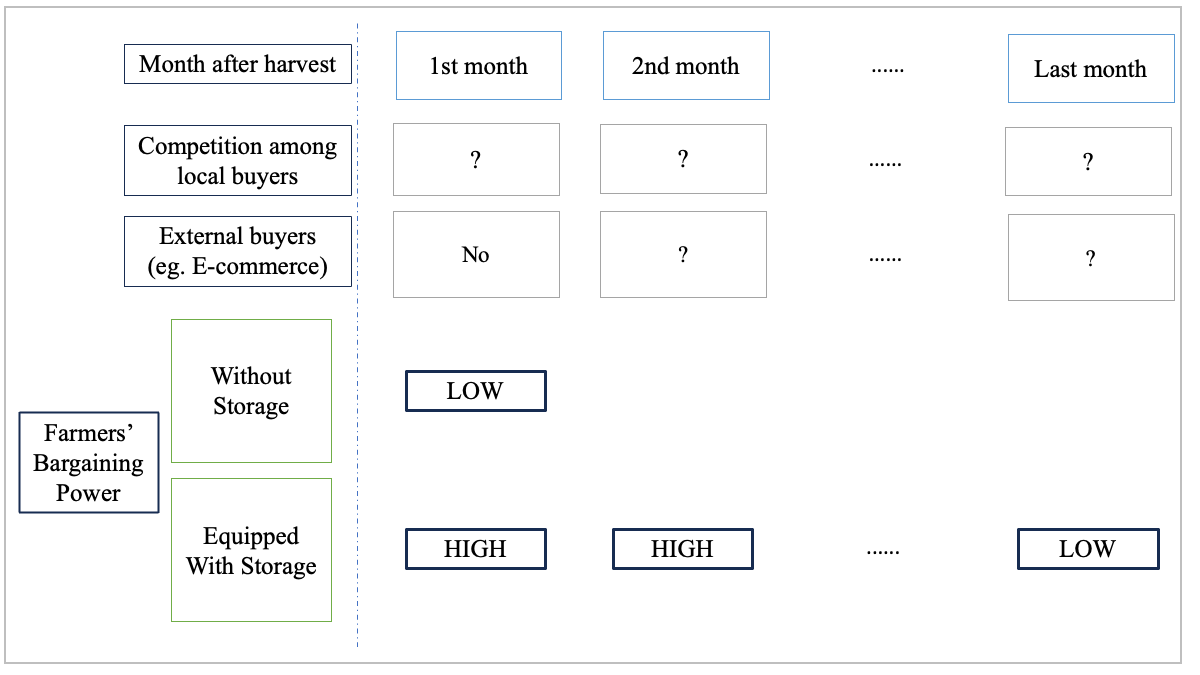
\includegraphics[width=1\textwidth]{figures/graphic_demo.png}
\caption{Extended Marketing Opportunities from Storage Adoption}
\label{Figure: Demo}
\end{figure}

Specifically, farmers could potentially benefit from increased competition in the oligopsonistic market through two sources. Firstly, the presence of different intermediaries in the village at various times can create fluctuating levels of competition on a monthly or even weekly basis. Secondly, farmers with storage can tap into additional distribution channels such as e-commerce and direct selling, which differ from the conventional middlemen-dominated system. By doing so, they can introduce external participants into the oligopsonistic market at the farm gate at different time nodes. 

I develop a conceptual framework to explore how smallholder farmers can adopt cold storage to potentially exploit the time-varying buyer power of middlemen. It considers a simplified dynamic, two-period scenario in a developing country, where farmers sell a specific cash crop to middlemen who visit local villages to procure the farm product. The model incorporates a storage-decision process, wherein farmers, observing farm-gate prices at harvest, decide whether to sell or store their crops.

The outcomes of this study hold substantial implications for policymakers and farmers alike. By exploring the dynamics of time-varying oligopsony levels, the research aims to demonstrate the potential benefits of storage facilities for smallholder producers. In a broader context, the findings suggest that embracing storage adoption could provide farmers with an effective alternative to combat anti-competitive practices like buyer collusion and market division and avoid more intrusive measures in markets, such as direct government intervention.





\section{Base Model}
\noindent I develop a two-period dynamic model to analyze how smallholder farmers strategically utilize storage in response to time-varying buyer power exerted by middlemen. The model is set in a rural area of a developing country, where farmers market a cash crop to itinerant traders. Harvest quantity is treated as exogenous, and the analysis focuses exclusively on farmers' storage and sales decisions within a single crop cycle. To identify the impact of market structure and trading dynamics, product quality is assumed homogeneous across farmers.

Farmers exhibit risk preferences ranging from risk neutrality to moderate risk aversion, valuing consumption at market prices. Each farmer is represented by a von Neumann–Morgenstern utility function,\footnote{An alternative mean-variance framework, presented in Appendix~\ref{Appendix: mean-variance approach}, yields similar insights. However, due to limited empirical guidance on calibrating the risk aversion coefficient within agricultural supply chains for the mean-variance framework, my primary analysis relies on the expected utility framework.} $U_i(\pi_i)$, with $U_i' > 0$ and $U_i'' \leq 0$, where $\pi_i$ is the farmer's net income from crop sales. Farmers aim to maximize the expected utility of income across two trading periods.

The central decision is determining the proportion of the harvest stored immediately post-harvest, denoted by $s \in [0,1]$. This choice is made under uncertainty about future market conditions, specifically future buyer power dynamics in the subsequent trading period. I will represent buyer power in each period $t$ by the parameter $\theta_t$ and will later show that we can bound $\theta_t$ in the unit interval.

In the initial trading period, farmers observe farm-gate price offers from middlemen. Based on the frequency and magnitudes of these offers, farmers infer the current buyer power. represented by $\theta_1$. Greater competition among buyers, characterized by lower $\theta_1$, correlates with higher farm-gate prices, $p_1$. Anticipating continuity in the inverse relationship between buyer power and prices across periods, farmers strategically allocate harvest between immediate sale and storage, incorporating expectations about future competition, captured by the random variable $\theta_2$.

Temporal demand variations downstream—such as seasonal consumption shifts—are presumed to be fully internalized by the market as a whole, including both farmers and intermediaries. Since intermediaries may engage in storage, anticipated demand fluctuations over the marketing season should already be reflected in the prices they offer at harvest. Accordingly, buyer power remains the primary source of intertemporal price variability in this model.

The model assumes symmetric information and negligible transaction costs in each trading period, ensuring farmers have complete and instantaneous access to prevailing farm-gate prices.

Formally, each farmer seeks to maximize expected utility over two trading periods by selecting storage share $s \in [0,1]$. Given a normalized harvest quantity $q = 1$, the optimization problem is:
\begin{equation}
\label{eq:starting objective}
\max_{s \in [0,1]} \mathbb{E} \left(U\left[ (1 - s) p_1 + s \cdot p_{2,\text{net}} \right]\right).
\end{equation}
where $p_1$ is the farm-gate price at harvest and $p_{2,\text{net}}$ is the second-period price adjusted for storage costs.



\subsection{Middlemen Market Structure and Farm-Gate Price Formation} \label{Section: Middlemen Market Structure and Farm-Gate Price Formation}
\noindent To analyze farmers' strategic use of storage as a form of intertemporal bargaining, it is essential to model farm-gate price formation in a manner that flexibly incorporates the degree of competition among middlemen.

I adopt the \textit{Flexible Oligopoly/Oligopsony Market (\textit{FOOM})} framework to model farm-gate pricing as a function of buyer market power. Under the assumption that downstream markets, wholesale or retail, where traders sell the farm products they procure, are perfectly competitive, the farm-gate price $p_{f,t}$ in each period $t$ is determined as:
\begin{equation}
p_{f,t} = \frac{p_{r,t} - mc_t}{1 + \frac{\theta_t}{\varepsilon_t}},
\end{equation}
where $p_{r,t}$ is the downstream price and $mc_t$ denotes the buyers' marginal cost in period $t$, $\theta_t$ captures the degree of buyer power in period $t$, and $\varepsilon_t$ represents the farm supply elasticity facing buyers in period $t$.\footnote{For a detailed derivation, see Appendix~\ref{Appendix: Derivation of Farm Price under the FOOM Framework}.}


for simplicity, supposing the downstream price net of marginal cost is constant across periods and normalizing it to unity ($p_{r,t} - mc_t = 1$), the farm-gate price reduces to:
\begin{equation}
p_{f,t} = \frac{\varepsilon_t}{\varepsilon_t + \theta_t}.
\end{equation}


Although total harvest quantity is fixed at the time of the first-period decision, supply in that period remains somewhat elastic due to farmers' ability to store part of their output. In period 2, supply is also elastic, as farmers can divert unsold produce to alternative buyers such as fruit-processing firms. To simplify the analysis while preserving these features, I assume a baseline supply elasticity of $\varepsilon_t = 1$ for both periods. This assumption serves as a plausible starting point and will be relaxed in subsequent analysis. Thus, farm-gate prices reduce further to:
\begin{equation}
p_{f,t} = \frac{1}{1+\theta_t}, \quad \theta_t \in [0,1],
\label{Eq: price formation by buyer power}
\end{equation}
where $\theta_t=0$ corresponds to perfect competition among buyers and $\theta_t=1$ denotes pure monopsony. Forms of oligopsony competition, such as Cournot competition, are represented by intermediate values of $\theta_t$, with higher values denoting progressively greater departures from competition \citep{karp1996dynamic,sexton2001assessment, saitone2009flexible, hamilton2021joint}.

Assuming farmers believe that this price formation rule persists across periods, period-specific prices are determined as $p_t = \frac{1}{1+\theta_t}, \quad t=1,2$. At harvest time, farmers observe $p_1$ and infer the contemporaneous buyer power, $\theta_1 = \frac{1 - p_1}{p_1}$. They then form expectations about the second-period buyer power, $\theta_2 \in [0,1]$, which is stochastic, and its distribution can be independent or based on the observation of $\theta_1$ under further assumptions. Thus, the second-period price can be expressed as:
\begin{equation}
p_2(\theta_2) = \frac{1}{1+\theta_2} 
\label{Eq: p_2 of buyer power change}
\end{equation}


To incorporate the economic cost of storage—including physical storage expenses, intertemporal discounting, and potential quality deterioration—I define the second-period price in net terms using a storage efficiency parameter $\kappa \in [0,1]$, which captures the overall storability of the commodity. Rather than modeling storage cost as a fixed deduction, I assume that storage frictions reduce the realized price proportionally, so that the farmer receives only a fraction $\kappa$ of the gross second-period price. This formulation captures a broad class of storage frictions, such as spoilage, shrinkage, and financing costs, that scale with the value of the commodity. It also reflects how farmers often perceive post-harvest losses: as a proportional reduction in potential revenue. From an analytical standpoint, the proportional specification preserves tractability under the Constant Relative Risk Aversion (CRRA) preferences, where utility is homogeneous of degree one and sensitive to relative rather than absolute changes in income. Accordingly, I define the net second-period price as:
$$
p_{2,\text{net}}(\theta_2) = \kappa \cdot p_2(\theta_2),
$$
where the gross second-period price remains $p_2(\theta_2) = \frac{1}{1 + \theta_2}$. Thus, the full expression becomes:
$$
p_{2,\text{net}}(\theta_2) = \frac{\kappa}{1 + \theta_2}.
$$
This setup ensures that the incentive to store responds coherently to economic fundamentals while allowing for an intuitive interpretation of $\kappa$: when $\kappa = 0$, the product is perfectly perishable and yields no second-period returns; when $\kappa = 1$, the product is perfectly storable with no loss in value.






\subsection{Final Objective Function}

\noindent The economic environment at harvest is summarized in Table~\ref{tab:baseline model parameter table}, capturing both observed and unobserved determinants of the farmer's storage decision over two periods.

\begin{table}[H]
\centering
\caption{Economic Environment at Harvest}
\label{tab:baseline model parameter table}
\begin{tabular}{lll}
\toprule
\textbf{Item} & \textbf{Symbol (units)} & \textbf{Status at Harvest} \\
\midrule
Harvest quantity & $q$ & Known, fixed (normalized to 1) \\
First-period price & $p_1$ & Observed \\
First-period buyer power & $\theta_1 = \frac{1 - p_1}{p_1}$ & Inferred from $p_1$ \\
Second-period buyer power & $\theta_2$ & Stochastic \\
Second-period price & $p_2 = \frac{1}{1 + \theta_2}$ & Derived \\
Storage efficiency factor & $\kappa \in [0,1]$ & Observed \\
Second-period net price & $p_{2,\text{net}} = \frac{\kappa}{1 + \theta_2}$ & Derived \\
CRRA risk aversion & $\gamma \in [0,1)$ & Observed \\
\bottomrule
\end{tabular}
\end{table}

\noindent The farmer allocates a share $s \in [0,1]$ of output to the second-period sale and retains the remainder for immediate sale at price $p_1$. Without a specific assumption on the utility functional form, substituting the expressions for $p_1$ and $p_{2,\text{net}}$, a farmer's maximization problem becomes:
\begin{equation}
\label{eq:final objective}
\max_{s \in [0,1]} \mathbb{E} \left\{U\left[\underbrace{\frac{1-s}{1+\theta_1}}_{\text{First-period income}} + \underbrace{s \cdot \frac{\kappa}{1+\theta_2}}_{\text{Adjusted second-period income}} \right]\right\}.
\end{equation}


\subsection{Risk Neutrality: Closed-Form Solution}
\noindent Under the case of risk neutrality, the utility function becomes linear: $U(\pi) = \pi$. The objective simplifies to:
\begin{equation}
\max_{s \in [0,1]} \; 
(1 - s) \cdot \frac{1}{1 + \theta_1} 
+ 
s \cdot \kappa \cdot \mathbb{E} \left[ \frac{1}{1 + \theta_2} \right].
\end{equation}
The solution simply depends on a comparison of marginal returns:
\begin{equation}
s^*( \gamma = 0) =
\begin{cases}
1 & \text{if } \kappa \cdot \mathbb{E} \left[ \frac{1}{1 + \theta_2} \right] > \frac{1}{1 + \theta_1}, \\
0 & \text{if } \kappa \cdot \mathbb{E} \left[ \frac{1}{1 + \theta_2} \right] < \frac{1}{1 + \theta_1}, \\
\text{any } s \in [0,1] & \text{if equality}.
\end{cases}
\label{Eq: risk-neutrality solution}
\end{equation}

\noindent Under risk neutrality, the farmer evaluates only expected monetary payoff. The decision reduces to a pure binary choice: if the net expected second-period price exceeds the normalized first-period price, then storage is optimal; otherwise, immediate sale dominates. Indifference arises only when the two expected returns are equal.


\subsection{Risk Aversion: Numerical Approach Needed}
\noindent In the presence of risk aversion—that is, when the utility function is strictly concave—analytical solutions to the farmer's maximization problem are generally out of reach. This intractability arises from the fact that risk aversion embeds the random second--period buyer–power shock $\theta_2$ inside a nonlinear transformation.  With a strictly concave utility function $U(\cdot)$, the marginal utility term that enters the first-order condition is $U'\!\left[\frac{1-s}{1+\theta_1}+ s\frac{\kappa}{1+\theta_2}\right]$.  Because $s$ appears both outside and inside the expectation, the optimality condition requires solving
$$
\mathbb{E}\!\left\{\,U'\!\Bigl[\cdot\Bigr]\!\left[-\frac{1}{1+\theta_1}+\frac{\kappa}{1+\theta_2}\right]\right\}=0,
$$
which is a Fredholm integral equation. For generic concave $U$ (e.g., CRRA, CARA, or quadratic utility outside the linear range), the integral has no closed-form anti-derivative, because $U'$ must be evaluated at every realization of $\theta_2$ and then averaged over its distribution. Only by imposing knife-edge assumptions—such as risk neutrality ($U''=0$), degenerate $\theta_2$, or special affine-transform utility—does the expectation reduce to an algebraic expression that can be inverted for $s$.

Even when the distribution of $\theta_2$ is simple, analytic integration remains elusive. The ratio $\kappa/(1+\theta_2)$ introduces a hyperbolic term inside $U$, so the composition $U'\circ g(\theta_2)$ usually lacks a primitive.  Consequently, the derivative of the expected utility cannot be written as a finite combination of elementary functions, precluding a closed-form solution for the interior optimum. 

Moreover, the introduction of risk aversion couples the mean and higher-order moments of $\theta_2$ together. The comparative-static effects of skewness or variance on $s^{*}$ therefore enter through higher-order derivatives of $U$, which are inseparable from the integral above.  This dependence further limits traceability.


These complications drive me to employ numerical analysis, specifically, the Monte Carlo evaluation of the expectation, to approximate the optimal storage share $s^{*}$ while respecting the corner constraints $s\in[0,1]$.





\section{Numerical Analysis} \label{Section: Base Model Numerical Analysis}
\noindent To examine how risk preferences and storage efficiency shape farmers' intertemporal marketing decisions under buyer power uncertainty, I numerically solve for the optimal storage share $s^*$ across a range of parameter values. This section describes the simulation design and computational procedure employed to approximate the farmer's decision problem under Constant Relative Risk Aversion (CRRA) utility.


\subsection{Setup and Parameterization}
\noindent A farmer is assumed to observe a moderate level of first-period buyer power $\theta_1 = 0.5$, the midpoint of the support. Second-period buyer power $\theta_2$ is stochastic and modeled using Beta distributions bounded on the unit interval $[0,1]$, allowing for flexible skewness and kurtosis while maintaining economically relevant support.

I consider eight distinct Beta distributions defined by a full factorial combination of:
\begin{itemize}
\item \textbf{Four means}: $\mu_{(\theta_2)} \in {0.2,,0.4,,0.5,,0.8}$, and
\item \textbf{Two variances}: $\sigma^2_{(\theta_2)} \in {0.02,,0.05}$, representing low and high uncertainty respectively.
\end{itemize}

For each $(\mu_{(\theta_2)}, \sigma^2_{(\theta_2)})$ pair, the corresponding shape parameters $(\alpha, \beta)$ are computed using the standard moment-matching formulas:

$$
\alpha = \mu_{(\theta_2)} \left( \frac{\mu_{(\theta_2)}(1 - \mu_{(\theta_2)})}{\sigma^2_{(\theta_2)}} - 1 \right), \quad
\beta = (1 - \mu_{(\theta_2)}) \left( \frac{\mu_{(\theta_2)}(1 - \mu_{(\theta_2)})}{\sigma^2_{(\theta_2)}} - 1 \right).
$$

I simulate 2,000 independent realizations of $\theta_2$ for each Beta distribution to approximate the expectation operator in the farmer's objective function.




\subsection{Numerical Strategy}
\noindent The computational approach exploits a simplification under risk neutrality ($\gamma = 0$). In this case, the utility function becomes linear and the farmer's decision reduces to the binary rule as shown in Equation~\ref{Eq: risk-neutrality solution}.

For all $\gamma > 0$, I numerically evaluate a farmer's utility under the Constant Relative Risk Aversion (CRRA) functional form:
\begin{equation}
U(\pi)=\left\{\begin{array}{ll}
\frac{\left(\pi^{1-\gamma}-1\right)}{(1-\gamma)} & \text { if } \gamma \neq 1 \\
\ln (\pi) & \text { if } \gamma=1
\end{array},\right.
\label{eq: CRRA}
\end{equation}
where $\gamma$ denotes the coefficient of relative risk aversion, and $\pi$ represents the net income realized over two periods. 

The adoption of the Constant Relative Risk Aversion (CRRA) utility function is supported by both theoretical appeal and empirical evidence. Theoretically, CRRA maintains a constant degree of relative risk aversion across income levels, aligning with microeconomic models of choice under uncertainty. Empirically, panel data studies consistently find that the share of risky assets in household portfolios remains stable across wealth levels—even amid substantial income fluctuations—supporting the CRRA assumption \citep{Berger2020Characterizing, chiappori2011relative, zavala2024unfair}. The unitless nature of the CRRA coefficient $\gamma$ enables meaningful comparisons of risk preferences across settings and countries \citep{Szpiro1986Relative, hardaker2000some}. A recent meta-analysis by \citet{Irsova2025Relative} finds that, after adjusting for publication bias, the average coefficient of relative risk aversion centers around 1 in general economic applications and between 2 and 7 in financial contexts—figures that align closely with my field observations.

Moreover, this utility form aligns well with observed farmer behavior in regions proximate to my study sites. For example, \citet{jin2024losses} document persistent risk-averse decision-making among apple growers in areas that substantially overlap with the geographic scope of my fieldwork.


To ensure the model remains broadly applicable beyond the context of apple production, I adopt a general range for the storage efficiency coefficient, $\kappa \in [0.6, 1.0]$, in the simulations. This parameter captures the combined effects of physical quality loss, storage costs, and intertemporal discounting.

For apple growers in particular, empirical evidence suggests that postharvest quality decline is modest within a single marketing season due to the use of cold storage, implying that quality deterioration is likely minimal. Storage costs are present but not prohibitive, and the dominant component affecting $\kappa$ may therefore be discounting. Drawing on literature from developing-country settings (e.g., \cite{frederick2002time, tanaka2010risk, bauer2012behavioral, saitone2018price, Belissa2019Liquidity, liu2020delayed, Umar2025Drivers}), relevant discount rates can be substantial, yet still consistent with values that keep $\kappa$ well above 0.6. Present bias is not considered here, as intra-seasonal decisions are assumed to follow time-consistent preferences. This range thus offers a realistic and flexible foundation for analyzing storage behavior under varying economic conditions.






\subsection{Simulation Grid}
\noindent Therefore, the numerical analysis is conducted over the following two-dimensional grid:
\begin{itemize}
\item \textbf{Risk aversion}: $\gamma \in [0, 10]$, discretized over 30 evenly spaced points.
\item \textbf{Storage efficiency}: $\kappa \in [0.6, 1.0]$, discretized over 20 points.
\end{itemize}

This design spans a broad range of economically plausible values—from risk neutrality to strong risk aversion, and from low to perfect storage efficiency.

Each candidate $s$ is evaluated over the 2,000 simulated values of $\theta_2$, and the resulting utilities are averaged to approximate expected utility. The maximizer of this set yields $s^*$ for the given $(\gamma, \kappa)$ configuration.

For each grid point $(\gamma, \kappa)$, I solve the farmer's problem by computing expected utility over a discrete set of 25 candidate storage shares $s \in [0, 1]$. The optimal share $s^*$ is the value that maximizes expected utility given the simulated distribution of $\theta_2$.



\subsection{3D Visualization and Interpretation}
\noindent To present results, I construct a 4-by-4 panel as shown in Figure~\ref{Figure:3D_formulation}. The layout is organized as follows:
\begin{itemize}
\item \textbf{Top and bottom rows} plot the probability density functions (PDFs) of the eight Beta distributions used to simulate $\theta_2$. Each panel is annotated with its corresponding $(\mu_{(\theta_2)}, \sigma^2_{(\theta_2)})$ and the implied $(\alpha, \beta)$.
\item \textbf{Middle two rows} display 3D surfaces of the optimal storage share $s^*$ as a function of $\gamma$ and $\kappa$, separately for low-variance (second row) and high-variance (third row) distributions.
\end{itemize}
Each 3D plot is rendered with a consistent viewing angle such that the origin, corresponding to the lowest values of both $\gamma$ and $\kappa$, appears closest to the observer. These simulation surfaces depict key mechanisms driving intertemporal storage and marketing choices under local market-structural uncertainty in agriculture.

\begin{figure}[pht]
\centering
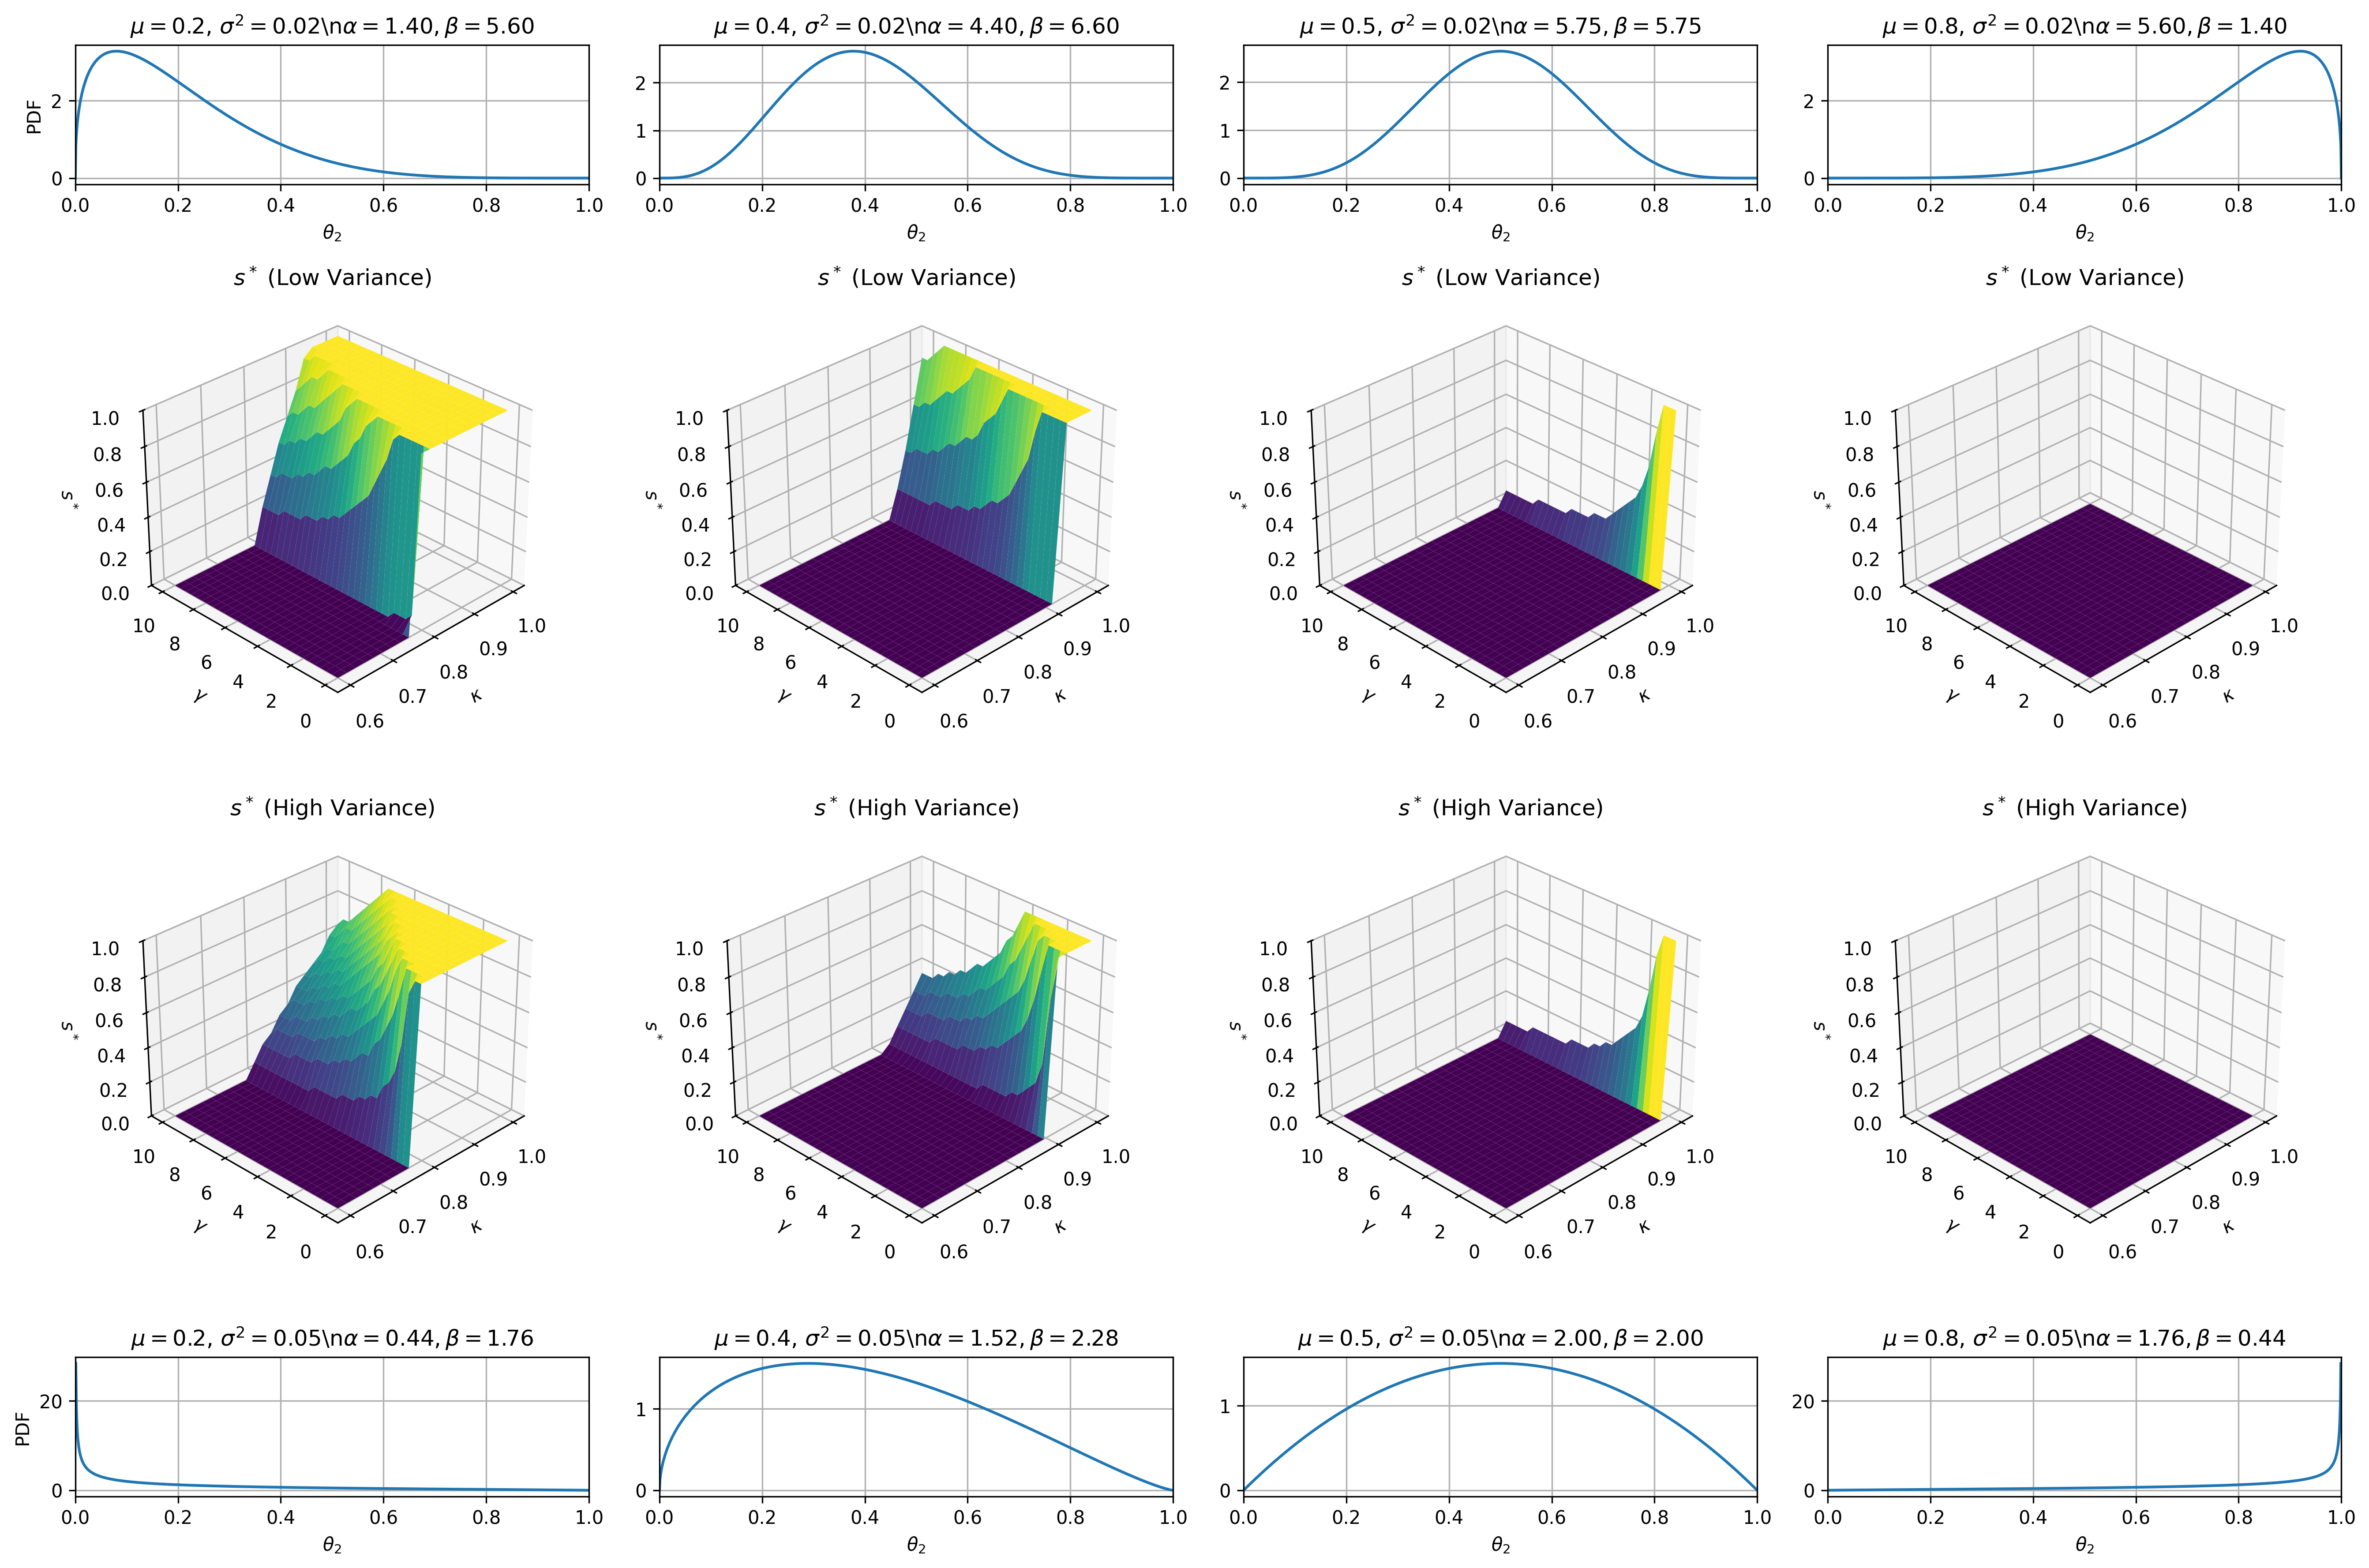
\includegraphics[width=\textwidth]{model_figures/3D_formulation.png}
\caption{Optimal Storage Share and PDF Visualizations under Eight Beta Distributions of $\theta_2$}
\label{Figure:3D_formulation}
\end{figure}

In general, when the farmer expects buyer power to be stronger in the future than at harvest—that is, when $\mathbb{E}[\theta_2] > \theta_1$—the incentive to store totally disappears. In other words, farmers would never store when $\mu > 0.5$ in our simulation here. As illustrated in the far-right column of the panel, the optimal strategy across all risk and efficiency levels is to sell immediately ($s^* = 0$).

In contrast, when expectations about future buyer power are neutral or favorable ($\mathbb{E}[\theta_2] \leq \theta_1$), the decision becomes more nuanced. Interior solutions ($0 < s^* < 1$) emerge over a meaningful range of risk preferences and storage efficiencies. Moreover, as the expected buyer power $\mathbb{E}[\theta_2]$ declines, both the scope for interior solutions and the frequency of corner solutions with full storage ($s^* = 1$) expand, reflecting the improved relative attractiveness of deferring sales.



Within each simulated surface, $s^*$ is non-increasing in $\gamma$. This pattern is especially pronounced when future buyer power is moderate—that is, when expected second-period prices are only marginally higher than those in the first period. The underlying mechanism is intuitive: risk-averse farmers increasingly value certainty over potentially higher but uncertain future payoffs. As $\gamma$ rises, the disutility associated with price risk begins to outweigh the intertemporal arbitrage opportunity, especially when those gains are compressed by relatively high buyer power.



In contrast, storage efficiency $\kappa$ plays a reinforcing role. For a given level of risk aversion, increases in $\kappa$ make storage more attractive by reducing the effective cost of waiting. Accordingly, $s^*$ is non-decreasing in $\kappa$, particularly when farmers are less risk-averse. The responsiveness of $s^*$ to $\kappa$ weakens at higher values of $\gamma$, suggesting that even highly efficient storage systems cannot fully offset the behavioral costs of risk exposure when farmers are strongly averse to uncertainty. 


Cross-panel comparisons further illustrate how changes in the distribution of second-period buyer power affect storage incentives. As the mean future buyer power $\mu_{(\theta_2)}$ increases (moving left to right across the panels), expected second-period prices decline, rendering storage less attractive in expected-value terms. Accordingly, the optimal storage share $s^*$ shifts downward across the entire surface. This effect is especially pronounced for risk-neutral or mildly risk-averse farmers, who condition decisions almost exclusively on expected returns. The lower the expected future price, the more immediate sale becomes the dominant strategy.



Variance in buyer power exerts a subtler influence. Comparing the second and third rows of the panel—low versus high variance cases—reveals that higher variance uniformly depresses $s^*$ across all parameter combinations. This effect reflects classical prudence: with concave utility, the marginal value of additional expected income diminishes in the presence of risk. Even when the expected second-period price remains high, increased dispersion in outcomes drives down the attractiveness of storage. The effect is pronounced at intermediate levels of $\gamma$, where farmers are sensitive to risk but not yet entirely averse to delayed selling.


\subsection{Rarity of Interior Solutions}
Interior solutions, where the farmer chooses to allocate positive fractions of the harvest to both the first and second periods, are theoretically rare in this model, tested from the simulation above. The logic is straightforward: when the intertemporal trade-off is starkly tilted in favor of one period (either due to price certainty, extreme risk preferences, or inefficient storage), the farmer's best response is to sell all in one period. This is consistent with fieldwork evidence in the fresh apple industry in Central China: most apple growers tend to make corner decisions, either storing nearly everything when they expect future prices to be favorable, or selling everything immediately when uncertainty or storage cost dampens the incentive to wait. Within the model, such corner solutions arise from the nonlinearity of the CRRA utility function combined with the hyperbolic dependence of price on buyer power, which amplifies small differences in expectations or attitudes into decisive action.

To better understand the conditions under which interior solutions might arise, I extract a few representative cases from the simulation results shown in Figure~\ref{Figure:3D_formulation}. These examples are selected from scenarios with low variance in second-period buyer power and a low mean, specifically $\mu = 0.2$, where the distribution of future prices is skewed toward favorable outcomes. We restrict attention to moderate levels of risk aversion and relatively high storage efficiency, where neither risk nor cost fully dominates the farmer's decisions.

The first case features a farmer with a risk aversion coefficient around $\gamma = 2$, a storage efficiency of $\kappa \approx 0.8$, and an expected buyer power of $\mu = 0.2$. Here, the farmer chooses to store approximately 80\% of the harvest. The low expected buyer power implies a high expected price in the second period, while the relatively efficient storage technology ensures that much of this value is preserved. The farmer, though risk averse, finds it worthwhile to defer income but hedges slightly by selling a small portion immediately. This aligns well with farmers who have moderate patience and access to good post-harvest storage infrastructure.

In the second case, the risk aversion parameter rises to $\gamma \approx 2.75$, with all other conditions held constant. The optimal storage share drops to about 62.5\%. The higher risk aversion amplifies the farmer's sensitivity to downside risk in second-period prices, even though the mean is favorable. The farmer still stores the majority, but the share sold in the first period increases. This behavior resembles that of more cautious farmers who hedge against worst-case outcomes even when market fundamentals appear strong.

The third case I select maintains the same level of risk aversion as in the second case ($\gamma \approx 2.76$) but reduces the storage efficiency to $\kappa \approx 0.68$. Under these conditions, the optimal storage share drops to roughly 45.8\%. The decline in $\kappa$ reduces the effective return to deferred sales, making immediate selling relatively more attractive. This farmer, facing the same preferences and expectations as in the previous case, responds not to belief or attitude but to technical constraint. It reflects real-world circumstances where storage facilities are substandard or subject to losses from spoilage, pests, or theft—conditions that naturally discourage holding output even among patient, forward-looking producers.

Together, these three cases illustrate the sharp responsiveness of the storage decision to both preferences and storage costs. As risk aversion increases, storage declines, all else equal. And for a fixed level of risk aversion, lower storage efficiency can easily shift the farmer from a moderately storage-heavy strategy to one that leans toward immediate sale. Crucially, these interior solutions emerge only under a narrow configuration of parameters: relatively favorable and stable expectations, moderate caution, and at least tolerable storage conditions. Once any of these dimensions shifts toward uncertainty, risk aversion, or storage economic inefficiency, the solution quickly reverts to a corner.

In summary, interior solutions occur only when multiple forces—expected price gains, risk preferences, and storage efficiency—are delicately balanced. These cases are not typical but represent transitional zones in the farmer's decision space. Their rarity in both theory and field data affirms the robustness of the model's prediction: for most farmers, especially under imperfect infrastructure and volatile markets, decisive corner choices are the norm.




\subsection{Sensitivity: Expected Future Buyer Power and Risk Aversion}
\noindent To further examine how a farmer's optimal storage share $s^*$ responds to varying expectations about future buyer power, I conducted a simulation with the same parameter setting as in the 3D graphics above by holding first-period buyer power fixed at $\theta_1 = 0.5$, with a storage efficiency of $\kappa = 0.9$. The second-period buyer power $\theta_2$ was modeled as a Beta-distributed random variable with support on $[0, 1]$, maintaining a fixed variance of 0.02 while allowing the mean to vary from 0.05 to 0.95. For each mean value, I derived the associated Beta shape parameters and simulated 5,000 draws of $\theta_2$. The optimal storage share was then computed by maximizing expected utility under CRRA preferences, evaluated across five levels of risk aversion: $\gamma \in \{0, 0.5, 2, 4, 7\}$. As shown in Figure~\ref{Figure: sensitivity to second-period buyer power}, each resulting function $s^*(\mathbb{E}[\theta_2])$ was plotted to visualize how forward-looking uncertainty and risk preferences jointly shape storage behavior. Line color was varied monotonically with $\gamma$, increasing in darkness as risk aversion intensified.

The results reveal a distinct shift in behavior across risk preference levels. Under risk neutrality ($\gamma = 0$), the decision rule is binary: the farmer stores all output if the expected net-storage-cost second-period price exceeds the current one, and none otherwise. As $\gamma$ increases to positive values, the decision becomes more nuanced. The sharp threshold gradually turns into a smooth, decreasing function of $\mathbb{E}[\theta_2]$, with interior solutions appearing when the expected future buyer power is only marginally lower than the first-period one.


With higher risk aversion (like $\gamma = 4$ and $\gamma = 7$), the willingness to store declines substantially. Even when the expected second-period price exceeds today's price, the farmer often chooses to sell immediately due to the downside risk embedded in the distribution of $\theta_2$. The curve $s^*(\mathbb{E}[\theta_2])$ flattens near zero, and the turning point at which storage becomes attractive shifts leftward. This leftward shift reflects a heightened preference for certainty: more favorable expectations are required before any intertemporal transfer of output becomes worthwhile. 


\begin{figure}[pht]
\centering
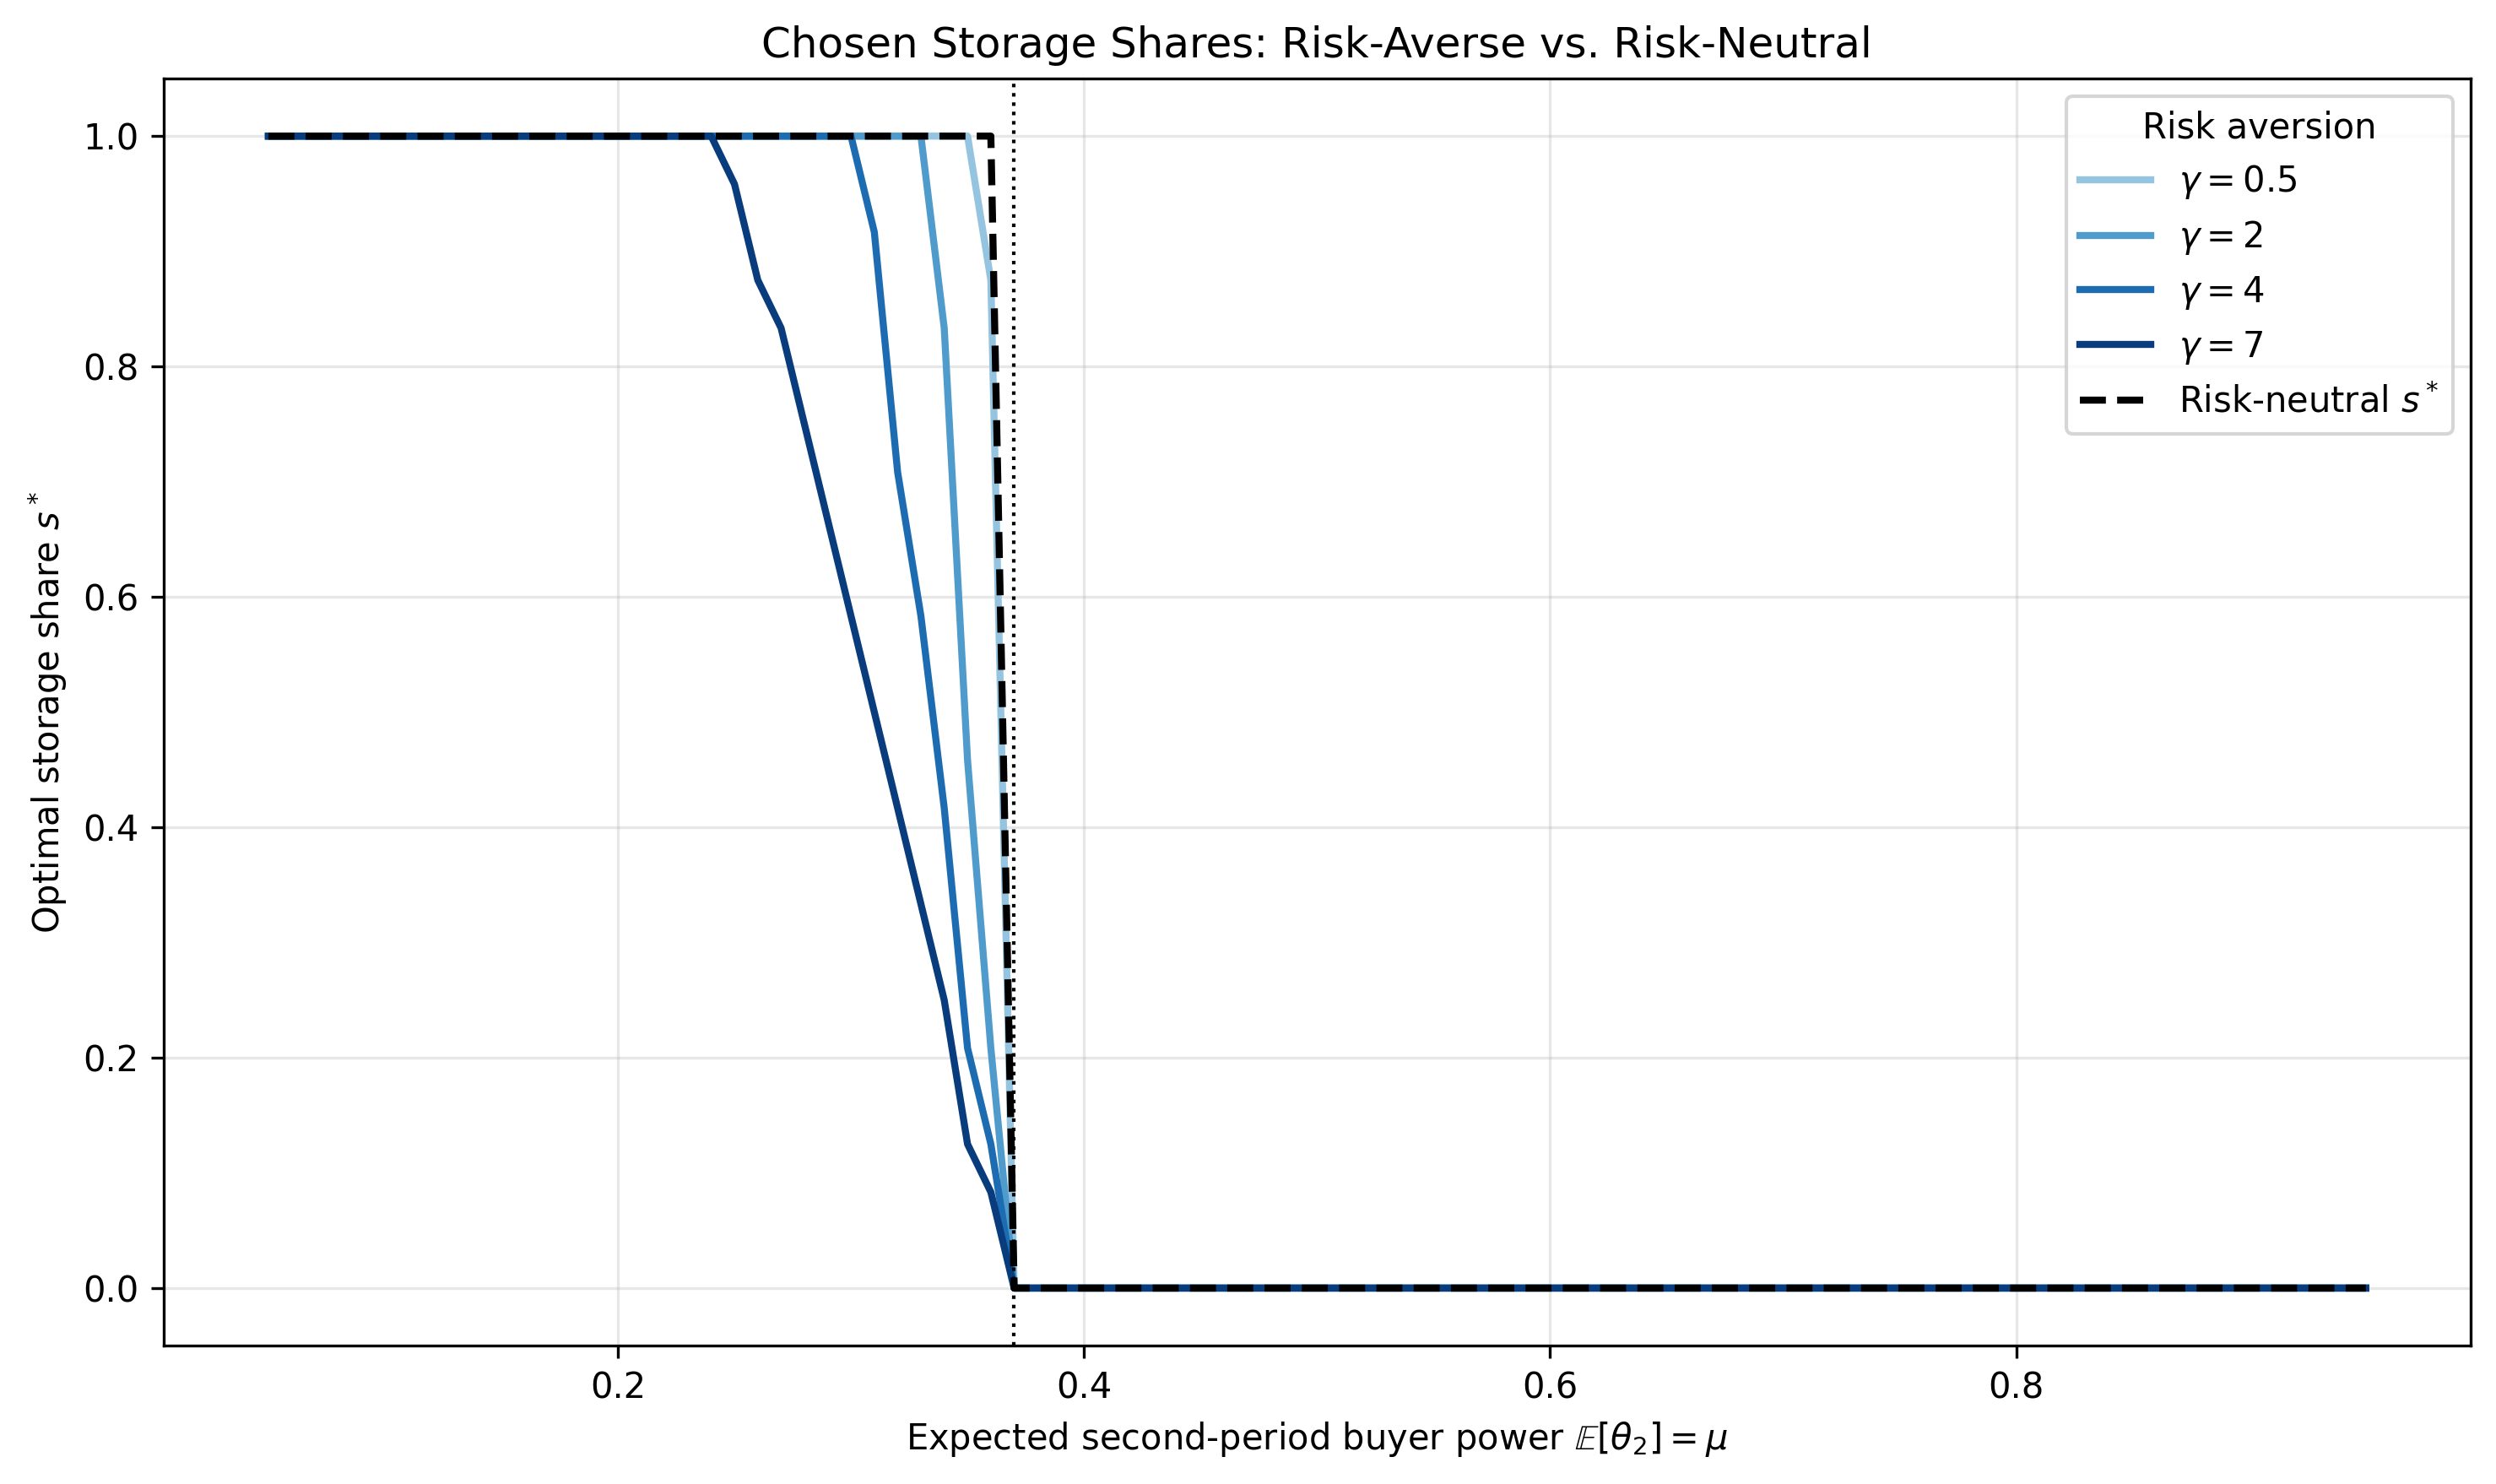
\includegraphics[width=\textwidth]{model_figures/sensitivity_to_theta_2.png}
\caption{Sensitivity to Expected Second-Period Buyer Power}
\label{Figure: sensitivity to second-period buyer power}
\end{figure}

\begin{figure}[pht]
\centering
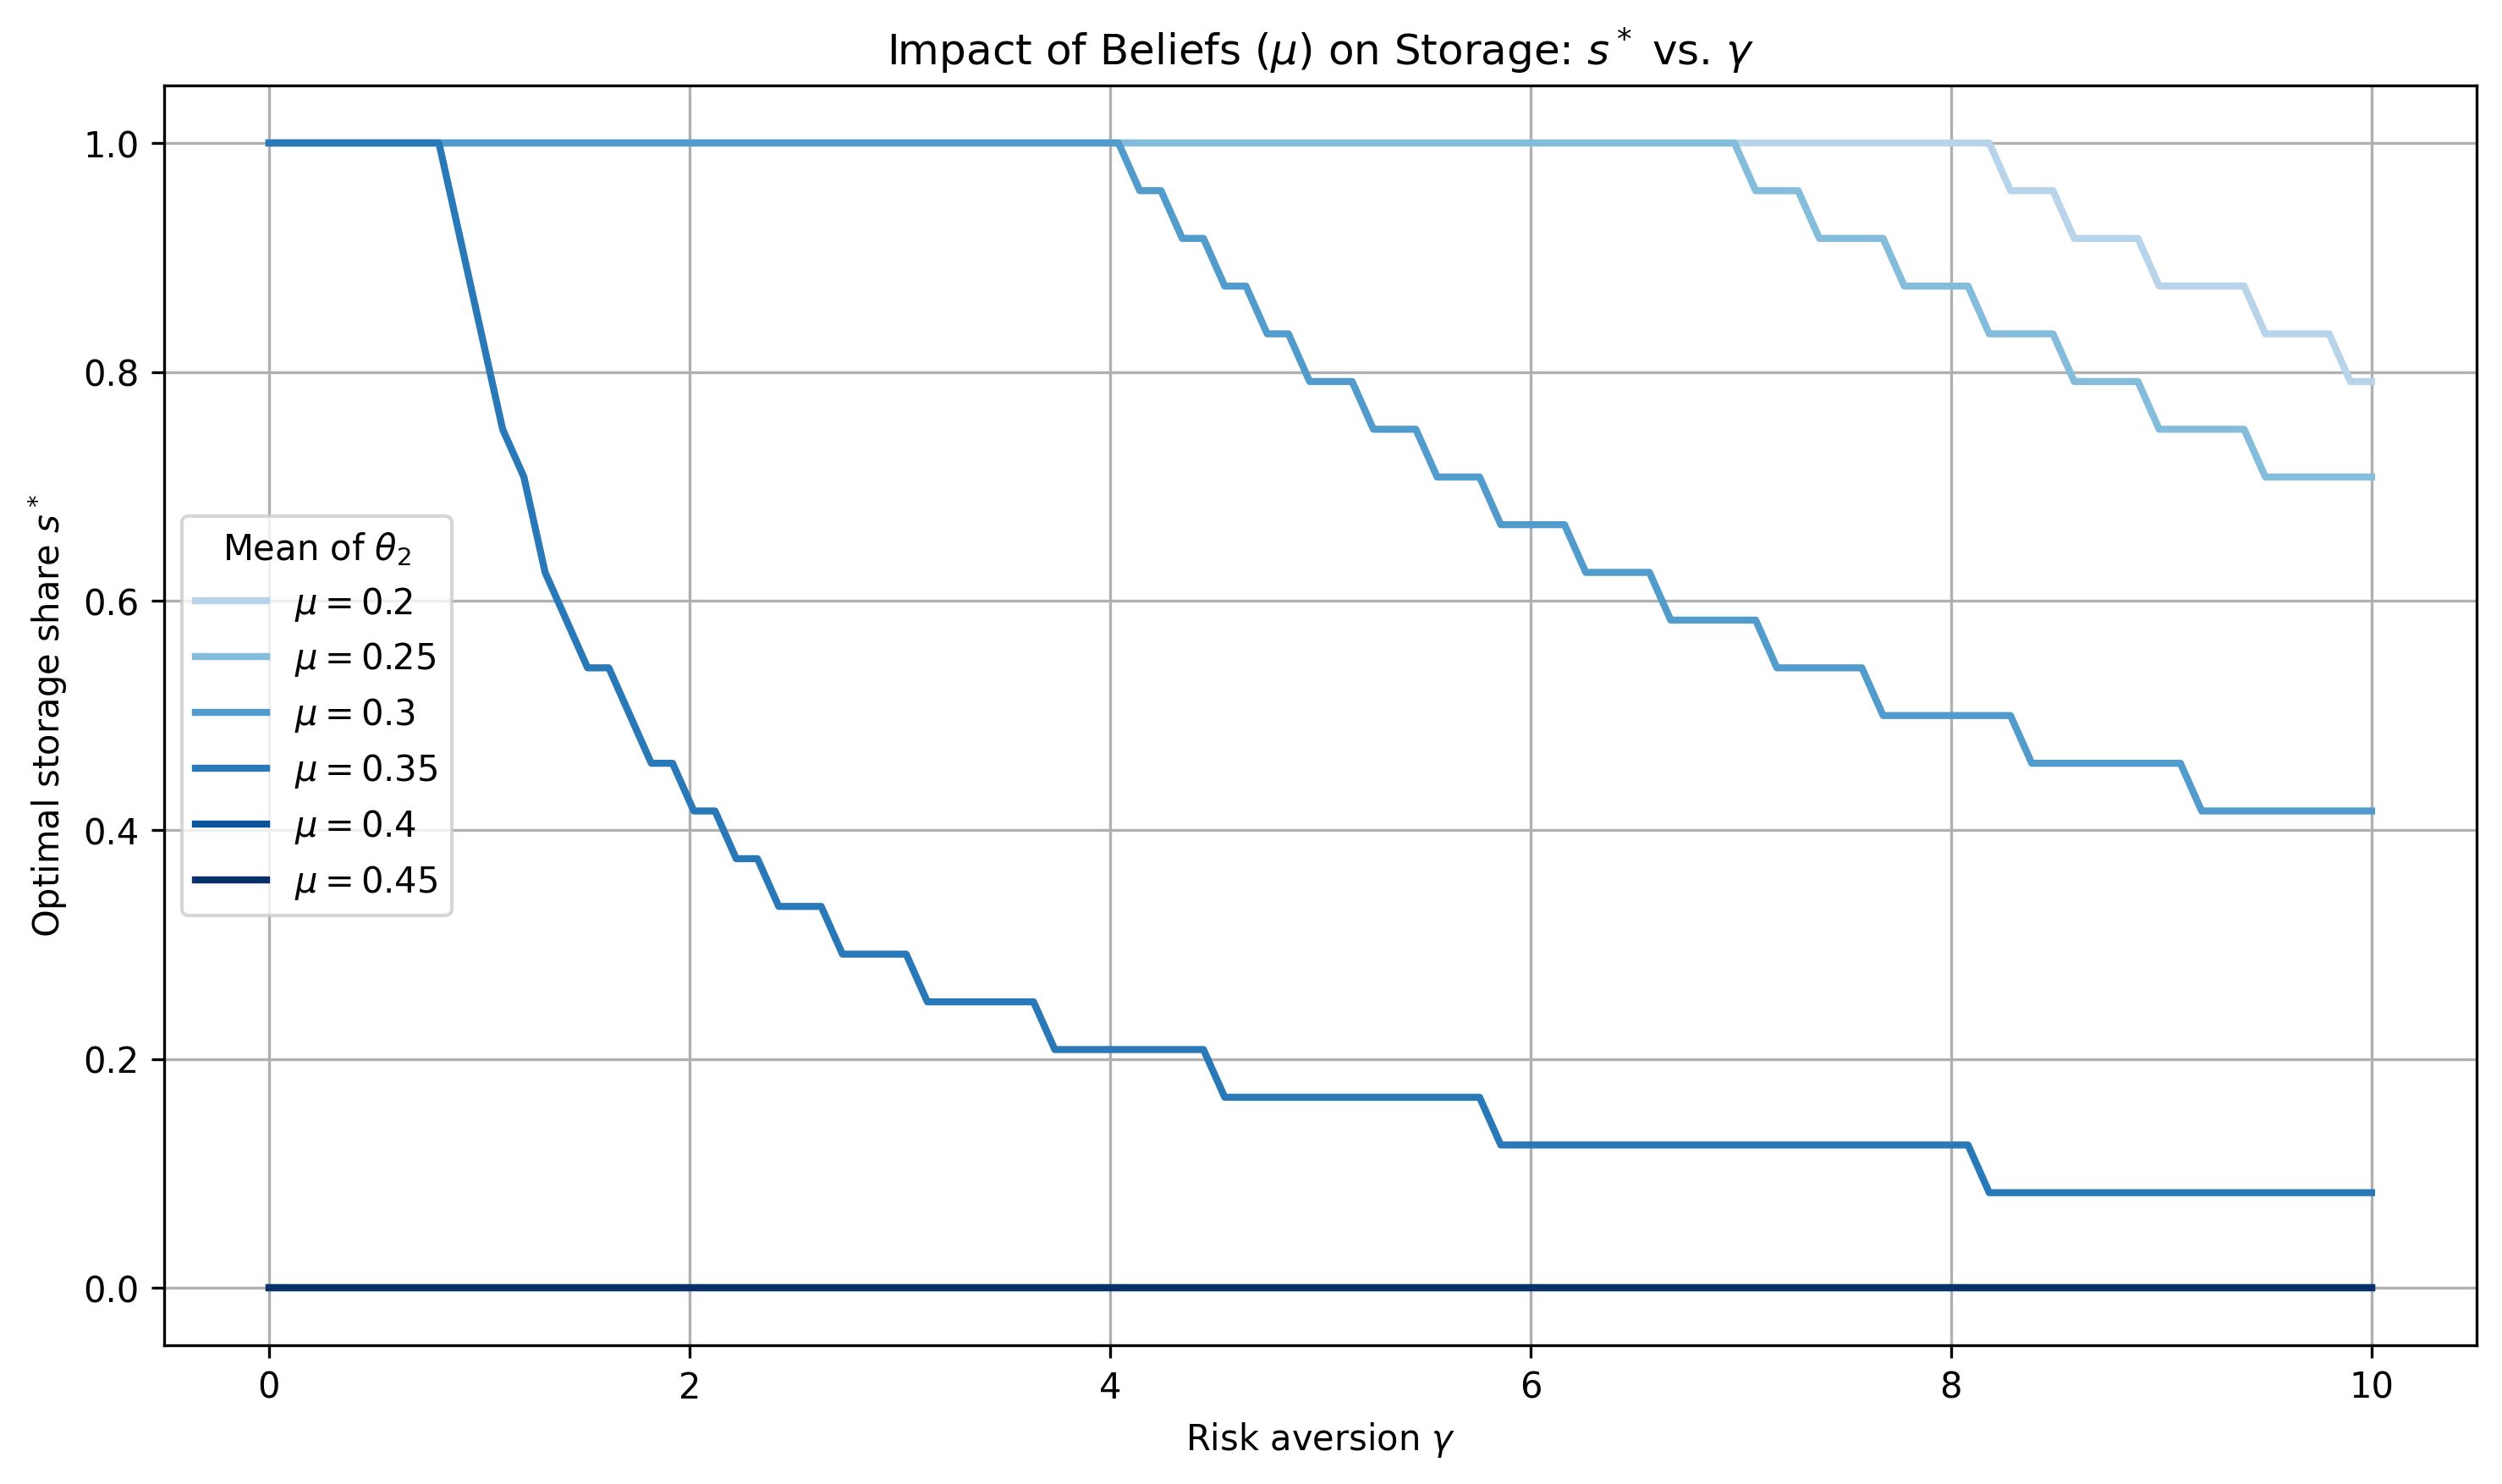
\includegraphics[width=\textwidth]{model_figures/sensitivity_to_gamma.png}
\caption{Sensitivity to Risk Aversion}
\label{Figure: sensitivity to risk aversion}
\end{figure}


In addition, I constructed another visualization in Figure~\ref{Figure: sensitivity to risk aversion} that examines how a farmer's optimal storage share responds to changes in risk aversion, under varying expectations about future buyer power. With the same parameter setting as in the 3D graphics above, I simulate buyer power beliefs using Beta distributions with means ranging from $\mu = 0.2$ to $\mu = 0.4$ in increments of 0.05. For each mean, I compute the corresponding shape parameters $(\alpha, \beta)$, draw 5,000 samples of $\theta_2$, and evaluate the expected utility under a CRRA utility function across 100 grid points of $\gamma \in [0, 10]$. The optimal storage share $s^*$ is computed by maximizing the expected utility over a grid of candidate values $s \in [0, 1]$, reflecting the proportion of harvest stored for second-period sale.



The resulting graph in Figure~\ref{Figure: sensitivity to risk aversion} plots $s^*$ against $\gamma$ for each value of $\mu$. Several patterns emerge clearly. First, storage shares are strictly decreasing in risk aversion: as farmers become more risk-averse, they prefer to sell more in the first period to avoid future price uncertainty. This is consistent with economic intuition, as risk aversion amplifies the penalty on uncertain second-period income. Second, higher expected buyer power in the second period (i.e., higher $\mu$) uniformly depresses the storage share. When future market power is expected to be strong (i.e., lower $p_2$), forward sales become less attractive, reinforcing the incentive to sell early regardless of risk preferences.

Interestingly, the sensitivity of $s^*$ to $\gamma$ becomes more pronounced as $\mu$ approaches $\theta_1$. For low $\mu$ (e.g., 0.2), storage is generally preferred—even by highly risk-averse farmers—because the expected second-period price is high. For higher $\mu$ values (e.g., 0.4), the curves flatten at lower levels of $s^*$, showing that even less risk-averse farmers opt for immediate sale under pessimistic price expectations.

This graphical structure complements prior results showing $s^*$ as a function of $\mu$ at fixed $\gamma$. Together, they offer a two-dimensional understanding of farmer behavior: beliefs about future buyer power shift the entire $s^*(\gamma)$ curve, while changes in risk aversion tilt its shape. These patterns are particularly relevant for understanding heterogeneous storage behavior across farmers who face similar market fundamentals but differ in attitudes toward risk or expectations about downstream market structure.



\section{Special Cases: Explicit Competition Forms}
\noindent In the base framework, buyer power was represented in a reduced-form manner typical of \textit{FOOM} models, where buyer power $\theta$ was treated as a latent, abstract variable inferred from observed farm-gate prices through a nonlinear transformation. Conceptually, $\theta$ can be thought of as a sufficient statistic for market structure and conduct: at one extreme, it may correspond to the number of downstream buyers $N$ (with higher $N$ implying weaker buyer power), while more generally it can capture the distribution of buyer market shares as well as the intensity of competition. For example, a low $\theta$ could reflect either many symmetric buyers competing aggressively, or a few large buyers that nonetheless compete rather than collude; conversely, a high $\theta$ could arise from concentrated market shares, tacit collusion, or explicit coordination. 

To move beyond this abstraction, I now introduce explicit models of non-cooperative buyer competition—namely, Bertrand (price-setting) and symmetric-buyer Cournot (quantity-setting) frameworks—thus ignoring for this analysis possible buyer collusion. These models provide structural microfoundations for $\theta$ by linking it to primitive features of market structure and strategic interaction.


Suppose farmers observe the number of buyers present in the village at harvest time in the first period, denoted by $N_1$, and form expectations about buyer presence in the second period, $\mathbb{E}[N_2]$. The number of buyers in each period is a discrete variable bounded between zero and a finite upper limit.

Bertrand and Cournot models offer contrasting benchmarks for non-cooperative buyer behavior. In the classic Bertrand setting, even a small number of buyers (as few as two) can generate highly competitive outcomes, a result often referred to as the ``Bertrand paradox.'' Translated into the present framework of traders purchasing from farmers, this implies that competition among a small set of buyers is sufficient to bid up the farm-gate price to the competitive benchmark—namely, the crop's \textbf{net marginal value product}, which by normalization equals 1.0 in the base model. In contrast, under Cournot competition the relationship between the number of buyers $N$ and the equilibrium farm-gate price is more gradual: as $N$ increases, buyer market power declines smoothly, and the farm-gate price converges to the competitive benchmark only asymptotically as $N \to \infty$.


To ground the discussion, I draw on my fieldwork among apple growers in Yanchang County, Central China, during the 2024–2025 agricultural year. According to my survey of the targeted 15 buyers, including the top five most influential local traders, the number of buyers visiting a village at harvest ranges from zero in remote areas to a maximum of nine.\footnote{In Figure~\ref{Figure: buyer count at harvest}, 26\% of farmers appear to forecast fewer than zero buyers in the future, which is clearly nonsensical. This artifact arises because my sample of 15 buyers does not exhaustively cover the entire population of potential buyers, only the majority of the most frequently observed ones. Hence, farmers expressing highly pessimistic expectations experienced buyer visits from buyers outside my sample.} The mean first-period buyer count is 3.34, with a median of 3. As shown in Figure~\ref{Figure: buyer count at harvest}, fewer than 7\% of surveyed growers reported no buyer presence during harvest (for simplicity, the Bertrand analysis excludes this case), while over 80\% experienced at least two buyer visits. Most farmers reported between two and five buyers, motivating my assumption of a Poisson distribution for second-period buyer counts in the Cournot analysis.

Importantly, farmers' expectations about second-period buyer presence appear weakly correlated with observed first-period buyer counts. This is illustrated by the color segments within each bar in Figure~\ref{Figure: buyer count at harvest}, which show considerable heterogeneity in forward-looking beliefs conditional on current buyer exposure.

\begin{figure}[hpt]
\centering
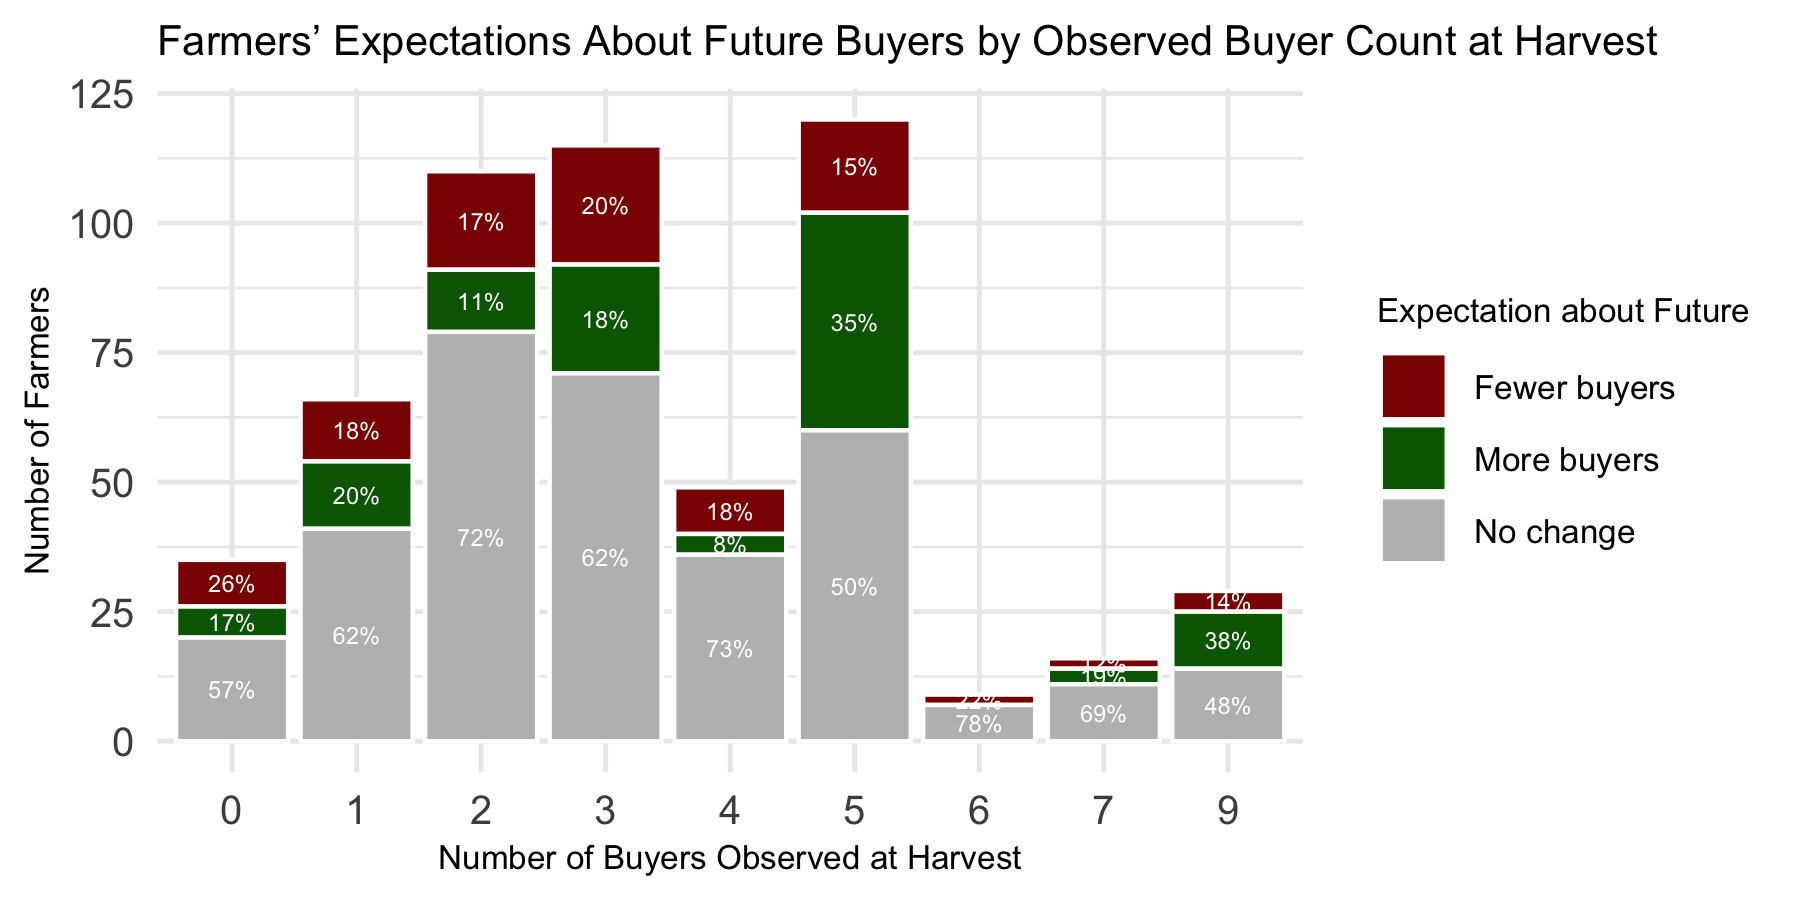
\includegraphics[width=\textwidth]{figures/buyer_count_distribution.png}
\caption{Observed Buyer Count at Harvest with Farmers' Expectations About Future Buyers}
\label{Figure: buyer count at harvest}
\end{figure}


\subsection{Price-Setting Competition: Bertrand--Nash Equilibrium}
\noindent In the price-setting environment, buyers choose the price at which they purchase from farmers. If there are no capacity constraints, the standard Bertrand logic applies: even two buyers suffice to drive the purchase price up to the competitive benchmark, which is normalized to 1 under our derived price formation rule in Section~\ref{Section: Middlemen Market Structure and Farm-Gate Price Formation}. This outcome, often referred to as the Bertrand Paradox, corresponds here to a Bertrand--Nash equilibrium in which perfectly competitive outcomes ($\theta_t=0$) arise as long as $N_t \geq 2$.

Therefore, under Bertrand conditions, according to Equation~\ref{Eq: price formation by buyer power}, the farm-gate price received by farmers can be modeled as:
\begin{equation}
p_t = 
\begin{cases}
0.5, & N_t = 1 \\
1, & N_t \geq 2
\end{cases}
\label{Eq: Bertrand Price Schedule}
\end{equation}
\noindent where $0.5$ denotes the monopsonistic price paid when only one buyer is present. The transition from a single-buyer market to a multi-buyer market results in a discontinuous shift in price.

Here, I assume that farmers observe the first-period price at harvest, and the number of traders at a specific village in the second trading period ($N_2$) is stochastic, with the probability of one middleman being $\rho$, i.e., $Pr(n_2=1)=\rho$. So, the probability of multiple intermediaries appearing in village $j$ is $Pr(n_2 \geq 2) = 1-\rho$. One plausible explanation for the temporal variation in buyer presence is the buyers' limited logistical capacity—such as a shortage of trucks or prohibitive transportation costs—which prevents them from visiting every village \citep{jung2022structural}. Another factor could be collusion among traders, leading to the allocation of markets, turning each trader into a monopsony in their assigned markets during the designated periods \citep{herings2005intertemporal}. However, collusion is prone to breakdowns, as cartels are inherently unstable. Therefore, even if trader collusion occurs in period 1, it may not persist into period 2.

Therefore, a farmer's optimization problem in Equation~\ref{eq:final objective} could be written as follows:
\begin{equation}
\label{eq:Bertrand objective}
\max_{s \in [0,1]} \psi(\cdot) = \rho U((1-s)p_1 + \kappa s \cdot 0.5) + (1-\rho) U \left( (1-s)p_1 +  \kappa s \cdot 1 \right)
\end{equation}
where the first expression on the right-hand side reflects the utility from storing $s$ share of production to the second period in the monopsonistic case, and the second term represents the utility in the case of perfect competition among buyers.

Differentiating Equation~\ref{eq:Bertrand objective} with respect to $s$ gives the marginal utility gain from reallocating one unit of output from immediate sale to storage:

\begin{equation}
g(\cdot) = \frac{d\psi}{ds} = \rho U^{\prime}(\pi_L(s)) \cdot (-p_1 + \kappa \cdot 0.5) + (1 - \rho) U^{\prime}(\pi_H(s)) \cdot (-p_1 + \kappa)
\label{Eq: bertrand FOC}
\end{equation}
where $\pi_L(s) = (1 - s)p_1 + \kappa s \cdot 0.5$ and $\pi_H(s) = (1 - s)p_1 + \kappa s$ denote net income under low and high second-period prices, respectively.

Evaluated at $s = 0$—i.e., no storage—the marginal utility becomes:
$$
\left.\frac{d\psi}{ds}\right|_{s=0} = U^{\prime}(p_1) \cdot \left[\kappa(1 - 0.5\rho ) - p_1\right]
$$
The bracketed term reflects the expected net second-period price, net of storage loss. Since $U'(\cdot) > 0$, the sign of this expression determines whether storing is utility-improving. In particular, the farmer finds storage profitable ($s^* > 0$) if and only if:
$$
\kappa(1 - 0.5\rho) > p_1
$$
That is, expected gains from delayed sale, adjusted for storage inefficiency, must exceed the current price. If this inequality holds, deviating from zero storage increases expected utility. Then we can derive the following three lemmas:
\begin{lemma}
    The condition $\kappa (1 - 0.5\rho) < p_1$ is necessary and sufficient for the farmer to sell the entire harvest in the first period, $s^*=0$.
        \label{lemma: Bertrand no storage solution}
\end{lemma}
\begin{proof}
    From Equation~\ref{Eq: bertrand FOC}, we can derive the second-order condition $\frac{d^2 \psi}{d s^2} = \rho U^{\prime \prime}\left(\pi_L(s)\right) \cdot\left(-p_1+ \kappa \cdot 0.5\right)^2+(1-\rho) U^{\prime \prime}\left(\pi_H(s)\right) \cdot\left(-p_1+\kappa\right)^2$. Since $U^{\prime\prime}(\cdot)\leq0$, the entire RHS expression is non-positive. Therefore, when $\kappa (1-0.5\rho) < p_1 $, the $\frac{d \psi(s=0)}{d s}$ would never be positive.
\end{proof}


\begin{lemma}
    On the contrary, when $\kappa (1-0.5\rho) > p_1 $ and $\frac{d \psi(s=1)}{d s}>0$, then the farmer maximizes utility by storing the entire harvest for second-period sale, $s^*=1$.
    \label{lemma: Bertrand full storage solution}
\end{lemma}
\begin{proof}
    As $\kappa (1-0.5\rho) > p_1 $ secures a positive storage share proven above, $\frac{d \psi(s=1)}{d s}>0$ ensures that expected utility is increasing in $s$. Therefore, at any given point of $s$, it would be optimal for the farmer to store more to get higher utility till $s$ reaches its upper bound.
\end{proof}


\begin{lemma}
    A farmer optimally adopts partial storage strategy (i.e., marketing production through both periods, $s^*\in (0,1)$) when the conditions $g(\cdot)  =  \frac{d \psi}{d s} = 0$ and $g^\prime(\cdot) = \frac{d^2 \psi}{d s^2} < 0 $ (implying a strictly risk-averse farmer), are satisfied in the range $0<s<1$.
    \label{lemma: Bertrand Interior solution}
\end{lemma}
\begin{proof}
    This is a standard interior optimum: the first-order condition holds and the second-order condition ensures a local maximum. Strict risk aversion ($U^{\prime\prime} < 0$) guarantees concavity and uniqueness.
\end{proof}

These three lemmas establish a complete characterization of the farmer's storage behavior: sell immediately, store fully, or split output across periods. Because the first-period price $p_1$ is itself endogenously determined by buyer competition (Equation~\ref{Eq: Bertrand Price Schedule}), we examine two benchmark cases: $p_1 = 1$ and $p_1 = 0.5$.

When multiple buyers are present at harvest, Bertrand competition drives the price to its competitive level, $p_1 = 1$. In this case, the expected second-period price, $\kappa(1 - 0.5\rho)$, falls below $p_1$, implying—by Lemma~\ref{lemma: Bertrand no storage solution}—that the farmer optimally sells all output immediately ($s^* = 0$). The benefit of immediate competition dominates any incentive to store.

In contrast, under monopsony at harvest ($p_1 = 0.5$), the storage decision becomes complex. The net gain from storing simplifies to $(\kappa -0.5)(1 - \rho)$, which is positive as long as: (i) the competitive price, adjusted for storage loss, exceeds the monopsonistic price; and (ii) there is a nonzero probability of facing competitive pricing in the second period ($\rho < 1$). Under these conditions, both full storage and interior storage solutions are feasible, depending on the form of risk aversion and specific parameter values.

Under monopsonistic first-period pricing, local comparative statics can be derived using the implicit function theorem. Let $g(s) = \frac{d\psi}{ds}$ denote the first-order condition for interior optimality. Then for any parameter $\xi \in {\rho, \kappa}$, the sensitivity of the optimal storage share satisfies:
$$
\frac{\partial s^*}{\partial \xi}= -\frac{\frac{\partial g}{\partial \xi}}{\frac{\partial g}{\partial s}}
$$
Since the second-order condition ensures $\partial g / \partial s = \frac{d^2\psi}{ds^2} < 0$, the sign of $\frac{\partial s^*}{\partial \xi}$ is governed by the sign of $\partial g / \partial \xi$. Hence, storage is increasing in storage efficiency factor $\kappa$—where lower storage cost unambiguously increases storage. However, the comparative statics with respect to $\rho$ is not signed deterministically. This limits the interpretive power of local sensitivity analysis, especially given the narrow parameter region where an interior solution $s^* \in (0,1)$ arises, as shown in the previous section.







\subsection{Quantity-Setting Competition: Cournot--Nash Equilibrium}
\noindent In the quantity-setting environment, each homogeneous buyer simultaneously chooses a purchase quantity, taking others' decisions as given. The resulting Cournot–Nash equilibrium reflects strategic quantity-setting behavior. Unlike in the Bertrand case, prices are not binary but vary smoothly with the number of active buyers.

Maintaining the linear demand structure introduced in Section~\ref{Section: Middlemen Market Structure and Farm-Gate Price Formation}, the farm-gate price in each period $t$ under quantity-setting competition is given by:
\begin{equation}
p_t = \max\left\{\frac{N_t}{N_t + 1}, \underline{p} \right\}, \quad t = 1,2,
\end{equation}
where $N_t \in \mathbb{N}_0$ denotes the number of standard fresh-fruit buyers in period $t$, and $\underline{p} \in (0,0.5)$ represents the low reservation price offered by fallback channels—typically processing facilities that accept any produce regardless of quality, but at steeply discounted rates. When at least one standard buyer is active ($N_t \geq 1$), the equilibrium price is strictly increasing in $N_t$, approaching the competitive limit of 1. When no such buyers are present ($N_t = 0$), the farmer receives $\underline{p}$ by selling to the outside option.

This formulation ensures continuity of the farmer's problem and captures the floor imposed by fallback markets. Although Figure~\ref{Figure: buyer count at harvest} includes a small number of reported instances with zero buyers, these are likely due to limitations in survey coverage, which focused on 15 standard fresh-fruit buyers and may have missed informal or processors' purchasing activity.

Accordingly, the farmer's maximization problem under Cournot competition becomes:
\begin{equation}
\label{eq:Cournot objective function}
\max_{s \in [0,1]} \mathbb{E} \left\{ U \left[ 
\underbrace{(1-s) \cdot p_1(N_1)}_{\text{First-period income}} 
+ \underbrace{s \cdot \kappa \cdot p_2(N_2)}_{\text{Adjusted second-period income}} 
\right] \right\},
\end{equation}
where $N_1$ is observed at harvest, $N_2$ is stochastic, and 
$p_t(N_t) = \max\left\{ \tfrac{N_t}{N_t + 1}, \underline{p} \right\}$ for $t = 1,2$. 


In simulation, I model second-period buyer availability $N_2$ as a discrete Poisson-distributed random variable truncated to the interval $[0,9]$, reflecting uncertainty over the presence of standard buyers while allowing for the possibility of no such buyers appearing. In the event that $N_2 = 0$, farmers can sell to a processing facility at a reservation price $\underline{p} = 0.1$, which serves as an outside option and places a floor on the farm-gate price. The first-period buyer count is fixed at $N_1 = 3$. As in Section~\ref{Section: Base Model Numerical Analysis}, farmers are assumed to exhibit constant relative risk aversion (CRRA) preferences.

Four different Poisson means, $\mu \in \{8, 6, 3, 1\}$, are considered, each representing different expectations about second-period market thickness. For each case, I simulated 5,000 realizations of $N_2$ and constructed a 2×4 panel plot in Figure~\ref{Fig: 3D Cournot}. The top row of the panel displays the probability mass functions (PMFs) of the Poisson distributions, illustrating how buyer count uncertainty is distributed under each mean. The bottom row presents 3D surface plots of the optimal storage share $s^*$ as a function of risk aversion $\gamma \in [0,10]$ and storage efficiency $\kappa \in [0.6, 1.0]$. The CRRA utility framework was applied, with a closed-form solution used when $\gamma = 0$. The results show that $s^*$ increases with both higher storage efficiency and lower risk aversion. Moreover, when the expected number of second-period buyers is low (e.g., $\mu = 1$), farmers optimally store less—particularly if they are risk averse.

\begin{figure}[htp]
    \centering
    \begin{subfigure}{\textwidth}
        \centering
        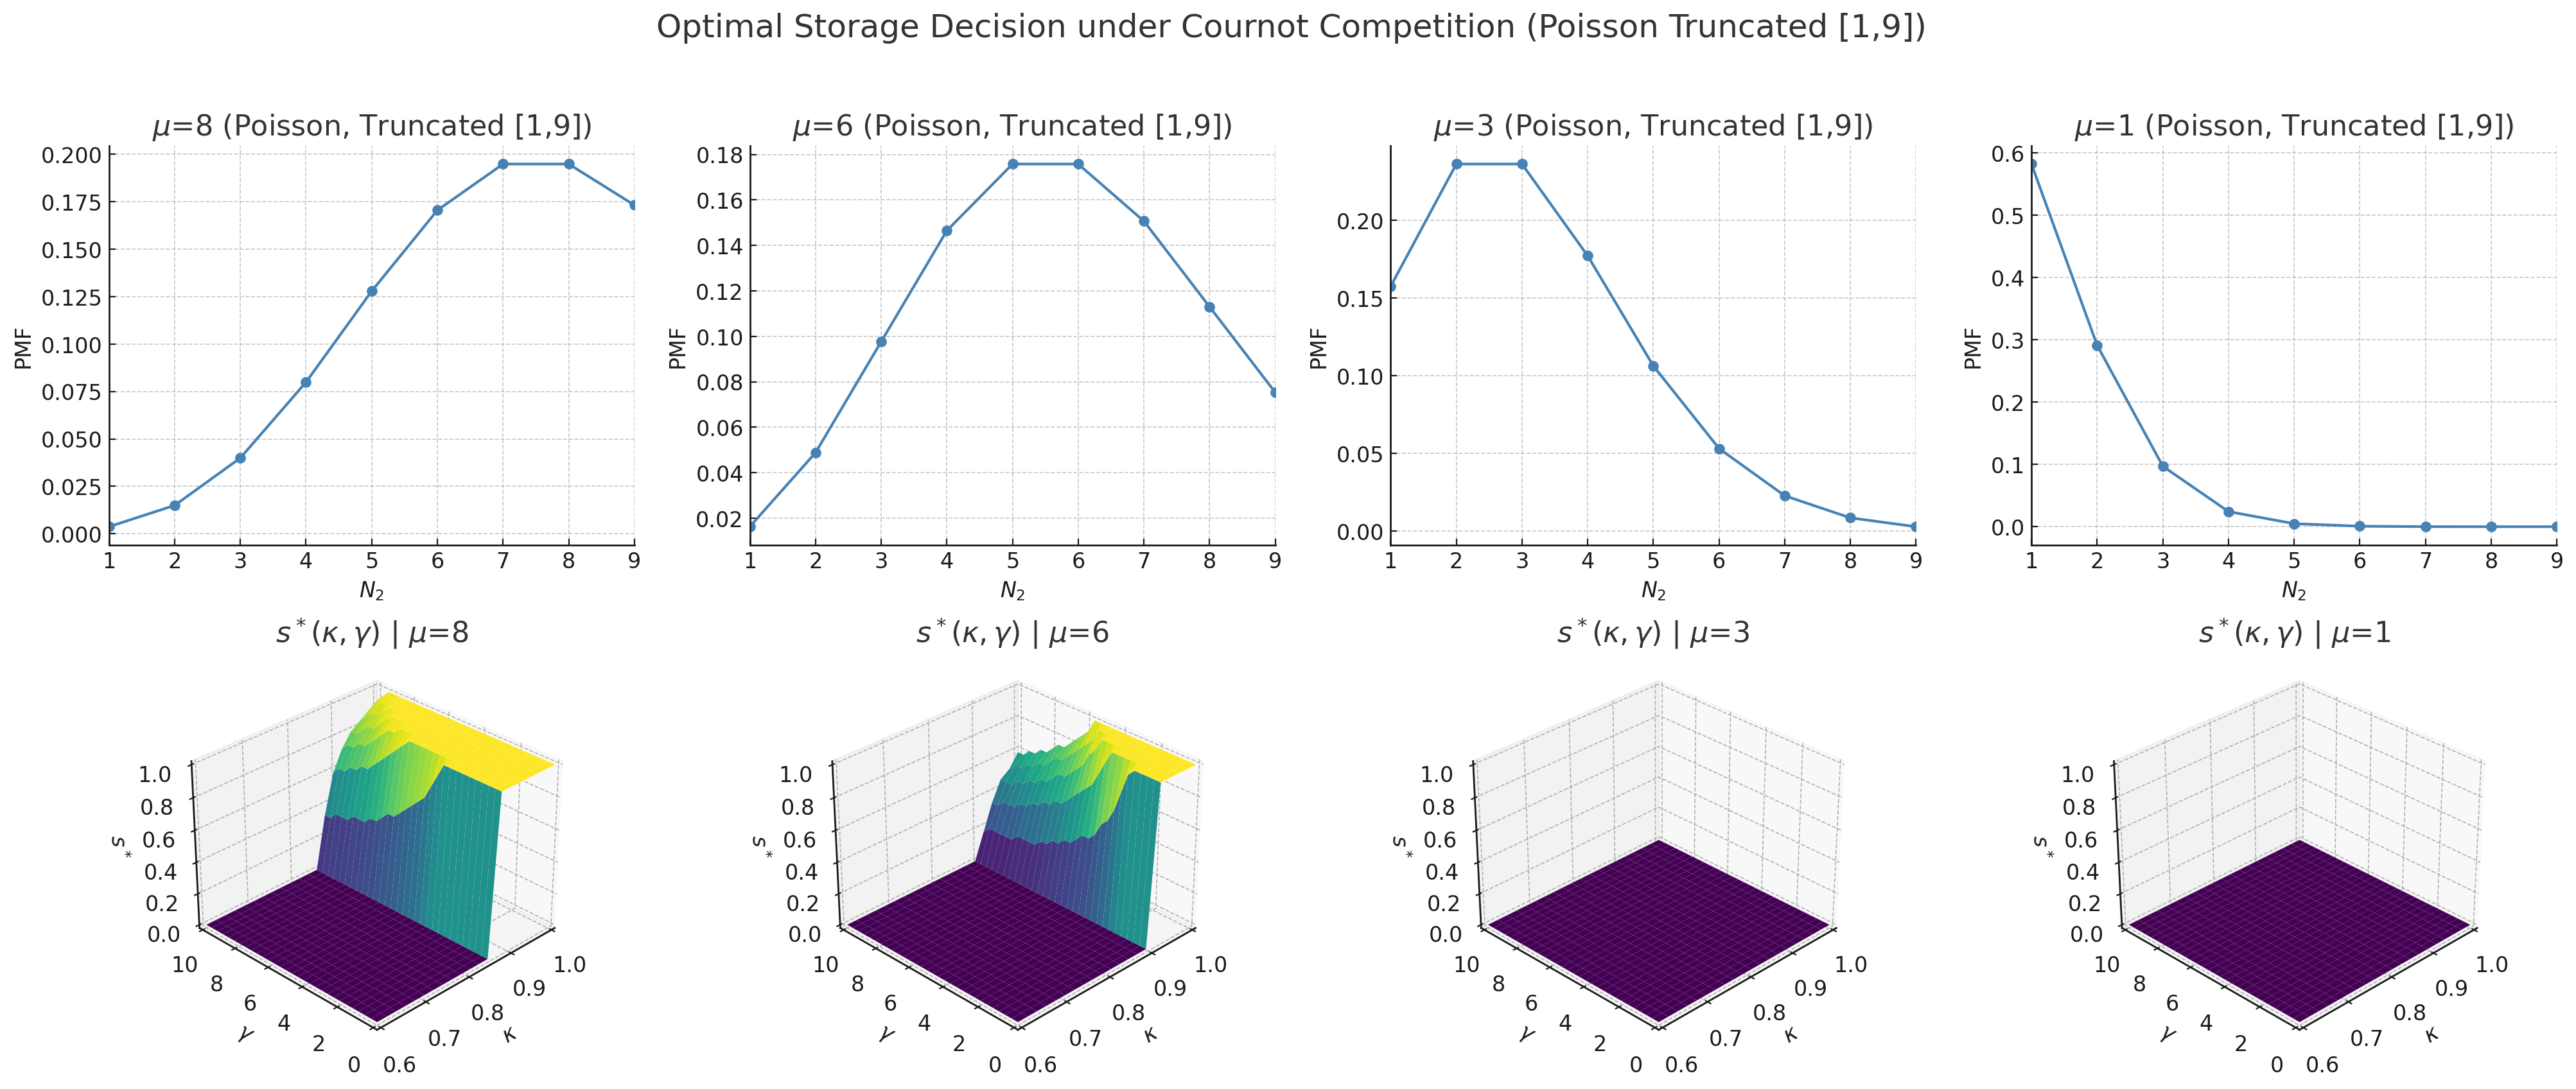
\includegraphics[width=\textwidth, keepaspectratio=true]{model_figures/3D_cournot.png}
        \caption{Optimal Storage Share and PDF Visualizations under Four Poisson Distributions of $N_2$}
        \label{Fig: 3D Cournot}
    \end{subfigure}
    
    \vspace{10mm} % Reduced vertical gap between subfigures
    
    \begin{subfigure}{\textwidth}
        \centering
        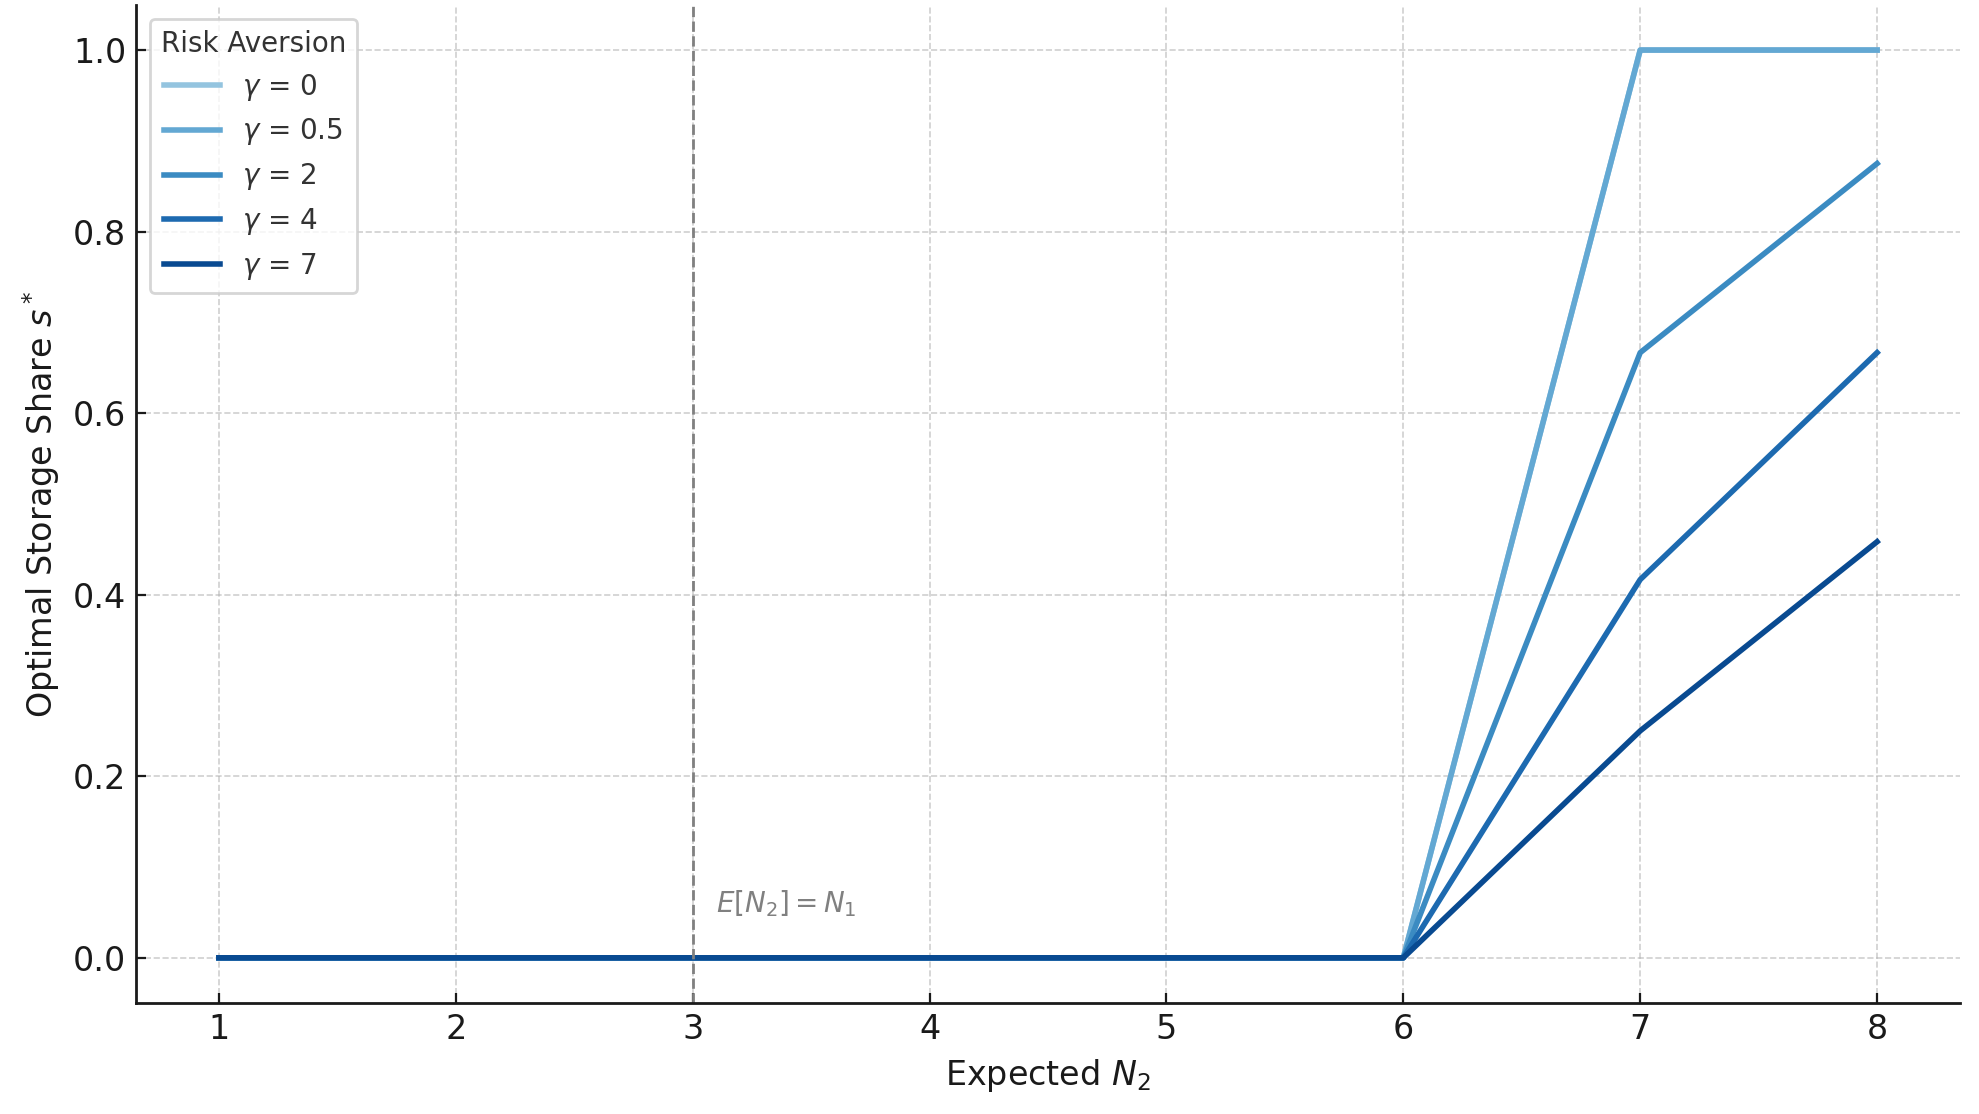
\includegraphics[width=\textwidth, keepaspectratio=true]{model_figures/buyer_count_sensitivity_cournot.png}
        \caption{Sensitivity to Expected Second-Period Buyer Presence ($\kappa=0.9$)}
        \label{Fig: Cournot sensitivity}
    \end{subfigure}

    \caption{Numerical Analysis under Cournot Competition}
\end{figure}



Figure~\ref{Fig: Cournot sensitivity} presents a three-panel sensitivity analysis of farmers' optimal storage share $s^*$ under Cournot competition when the second-period number of buyers follows a truncated Poisson distribution on $[0,9]$. The horizontal axis in each panel reports the expected value of $N_2$, and the vertical axis shows the corresponding optimal storage share. Each curve traces $s^*$ for a different level of risk aversion $\gamma \in \{0,0.5,2,4,7\}$, with darker shades of blue indicating higher $\gamma$. A vertical dashed line marks the benchmark case where the expected number of second-period buyers equals the observed first-period value, $\mathbb{E}[N_2]=N_1=3$. The three panels vary the assumed reservation price floor, $p_{\mathrm{reserve}} \in \{0.10,0.25,0.40\}$, which represents the outside option available if no standard buyers are present. This design allows direct comparison of how the outside option shifts storage incentives across risk preferences and market competitive scenarios.

Introducing a reservation price $p_{\text{reserve}}$ shifts the whole schedule upward in a economically intuitive way. A better fallback (from $0.10$ to $0.25$ to $0.40$) weakly lowers the threshold $\mathbb{E}[N_2]$ at which storage becomes attractive and increases $s^*$ at any given $\mathbb{E}[N_2]$—with the effect most pronounced for high $\gamma$, because the floor insures the downside of thin buyer markets. In short: more expected buyers and a stronger outside option both raise the optimal storage share, while greater risk aversion tempers that response.

On any particular curve plot in Figure~\ref{Fig: Cournot sensitivity}, for all $\gamma$, $s^*$ increases as the expected second-period buyer count rises, reflecting improving market prospects. More risk-averse farmers (higher $\gamma$) are generally less willing to store unless second-period conditions are significantly better than the present.

A key insight is that even under relatively favorable conditions—such as a low composite storage cost ($\kappa = 0.9$) and a moderately competitive harvest market ($N_1 = 3$)—storage becomes an attractive option only when farmers anticipate a substantially more buyer-presence market in the second period. Specifically, storage is only worthwhile when the expected number of buyers in period 2 reaches or exceeds 6, implying an expected price increase from $p_1 = \frac{3}{4} = 0.75$ to $p_2 = \frac{6}{7} \approx 0.857$. This 10.7 percentage point gain is sufficient to offset the 10\% effective loss due to storage inefficiency.


This result reflects the concave nature of the price function $p(N) = \tfrac{N}{N+1}$: as $N$ increases beyond 3, marginal improvements in price diminish. Therefore, even risk-neutral farmers require a strongly optimistic expectation of increased buyer presence to justify intertemporal arbitrage through storage. 

By contrast, when $N_1$ is very small (e.g., 1 or 2), the incremental price gains from attracting just one or two additional traders are much larger. For instance, moving from $N_1=1$ to $N_2=2$ raises the farm-gate price from $p_1=\tfrac{1}{2}=0.50$ to $p_2=\tfrac{2}{3}\approx 0.67$, while moving from $N_1=2$ to $N_2=3$ increases it further to $p_2=\tfrac{3}{4}=0.75$. Such discrete jumps can be large enough to incentivize storage. Thus, the stark threshold effect documented above is most relevant when the harvest market already exhibits moderate competition.





%----------------------------------------------------%
%----------------------------------------------------%


\section{Further Extensions}

\subsection{Other Models of Risk Preference}
\noindent According to \cite{o2018modeling}, "Real-world risk aversion is clearly not as straightforward as expected utility suggests. Additional sources of risk aversion (or risk-seeking) need to be used instead of, or in conjunction with, diminishing marginal utility of wealth." Individuals assess options involving both gains and losses, the "kink" in the value function between losses and gains induces risk aversion. Therefore, future researchers may extend my model by exploring the Loss Aversion models \citep{kahneman1979prospect}, in addition to the expected utility theorem. The approach developed by \cite{kHoszegi2006model, kHoszegi2007reference, kHoszegi2009reference} in addressing loss aversion with an endogenous reference point aims to mitigate this degree of freedom by asserting that the reference point is entirely determined by one's expectations about outcomes. Despite this, there has been limited progress in adapting alternative models to dynamic settings, with a notable exception of \cite{kHoszegi2009reference}, who define loss aversion concerning changes in beliefs regarding both current and future consumption.


\subsection{Collective-Action Dilemma: The Storage "Treadmill"}
\noindent Field observations suggest a collective-action dilemma surrounding storage adoption. As more farmers in a village adopt storage, middlemen may redirect procurement efforts to neighboring villages with less storage penetration, where farmers face weaker bargaining positions. This strategic shift reduces buyer competition at harvest in the original village, particularly disadvantaging farmers without storage. Consequently, even those initially indifferent to storage face mounting pressure to invest, not necessarily for higher profits, but to avoid worsening terms of trade. This dynamic mirrors the classic ``technology treadmill'' described by Cochrane \citep{cochrane1958farm, levins1996treadmill}, wherein early adopters gain temporary advantages that vanish as adoption becomes widespread, ultimately forcing others to follow suit merely to stay even. Future extensions of the model could incorporate this endogenous spillover—possibly via a parameter capturing buyer response to aggregate storage rates—highlighting how individually rational behavior may generate suboptimal collective outcomes.


\subsection{Non-linear Storage Cost}
\noindent Storage costs for farmers, defined as the sum of the actual cost of renting or operating storage space and the cost of deterioration, could be non-linear in many cases. For perishable goods like apples, the primary reason for convex storage costs is probably that spoilage and quality deterioration increase over time. Also, the operating costs of storage may not increase linearly with the volume of goods stored. Managing temperature and humidity conditions for larger quantities might require more sophisticated technology and energy consumption, leading to non-linear cost increases.

Supporting this notion, \cite{williams1989economic} demonstrates, through a quadratic form of total marketing costs, that farmers need to weigh the marginal revenue of later sales against the elevated costs incurred. This balance leads to a positive inventory, even without considering risk aversion. Instead of capturing the composite storage cost by a discounting factor, a well-designed mathematical model would allow other forms of storage costs, therefore, may give us other relevant real-world policy implications.


\section{Policy Implications}
\noindent
Whether in developing or advanced economies, policymakers care deeply about farm incomes. A common response has been direct interventions, such as minimum support prices or income transfers, that boost incomes but often at the cost of market distortions, fiscal burden, and misallocation of resources. The model here suggests an alternative emphasis: improve the environment in which farmers make intertemporal selling decisions. Three margins emerge from the analysis, competition, storage efficiency, and risk aversion, each capable of lifting expected incomes without direct price manipulation.



\subsection{Enhancing Competition among Buyers}

\textbf{Mechanism.} When competition among buyers is weak at harvest, farmers face low farm-gate prices. In the model this is captured by a high $\theta_1$, which depresses the immediate return to selling. Storage provides farmers with the option value of waiting, and its payoff rises if competition is expected to be stronger in the future, i.e.\ when the mean of $\theta_2$ falls and the second-period price distribution shifts upward. In this way, stronger future competition amplifies the benefits of storage by improving the relative return to waiting rather than selling at harvest.

\textbf{Quantitative illustration ($\delta=1$, $\kappa=0.9$, $\text{Var}(\theta_2)=0.02$):}
\begin{itemize}
  \item Suppose $\theta_1=0.5$ (harvest price $p_1=0.667$) and beliefs about buyer power shift from $\mu=0.37$ (weaker future competition) to $\mu=0.32$ (stronger future competition). Risk-neutral and risk-averse ($\gamma=2$) farmers both switch from \emph{no storage} to \emph{full storage}. Expected income rises from $0.667$ to $0.690$, a gain of $+\;0.023$.
\end{itemize}

\textbf{Policy interpretation.} When policy succeeds in enhancing competition at harvest, the immediate farm-gate price $p_1$ rises, improving farmer welfare unconditionally. In this case, storage functions less as an active strategy and more as a bargaining tool: the mere possibility of deferring sales deters monopsonistic buyers from pushing down harvest-time prices. More importantly, the model also shows, however, that such policies may not always generate an immediate effect at the start of each marketing season. As long as competition among buyers improves later in the season, storage enables farmers to arbitrage this dynamic change, raising expected incomes even when they are risk-averse. Policy instruments that can deliver these gains include stricter antitrust enforcement to deter collusion, lowering entry barriers for new traders, and investing in digital trading platforms or logistics infrastructure that broaden farmers’ access to alternative buyers over the marketing season.





\subsection{Subsidizing Storage and Technology Adoption}

\textbf{Mechanism.} The model shows that improving storage efficiency---captured by a higher $\kappa$---raises the net return from delaying sales. In practical terms, farmers retain more value from what they store, making the option to wait more attractive. This effect is particularly strong when market conditions are finely balanced, because even a modest improvement in storage efficiency can shift farmers from selling immediately to storing their entire harvest.

\textbf{Quantitative evidence (fix $\theta_1=0.5 \Rightarrow p_1=0.667$, $\delta=1$, $\text{Var}(\theta_2)=0.02$; raise $\kappa$ by 10\% from $0.90 \to 0.99$):}
\begin{itemize}
  \item At $\mu=0.33$, risk-neutral farmers already store fully, but expected income still rises markedly from $0.684$ to $0.752$ ($+\;0.068$).
  \item At $\mu=0.35$, risk-neutral farmers continue to store fully, while moderately risk-averse farmers ($\gamma=2$) increase storage from 50\% to 100\%; their expected income rises from $0.670$ to $0.741$ ($+\;0.071$).
  \item At $\mu=0.37$, right at the margin, both risk-neutral and risk-averse farmers switch from no storage to full storage, with expected income increasing from $0.667$ to $0.730$ ($+\;0.063$).
\end{itemize}

\textbf{Policy interpretation.} A 10\% increase in storage efficiency yields substantial income gains---on the order of 6--7 percentage points---and can induce dramatic behavioral shifts in storage, especially near the decision boundary. These results suggest that policies which subsidize storage or promote better technologies (e.g., air-controlled cold storage, or improved post-harvest handling) can deliver sizable welfare benefits without distorting market prices. Unlike direct price supports, which are costly and often inefficient, improving $\kappa$ raises returns across the board and strengthens farmers’ ability to capture intertemporal gains from storage. 






\subsection{Reducing Effective Risk Aversion via Financial Deepening}

\textbf{Mechanism.} While intrinsic risk preferences are relatively stable, \emph{effective} risk aversion declines as farmers gain financial security through liquidity, insurance, and wealth accumulation. A lower coefficient of relative risk aversion ($\gamma$) shifts behavior toward the risk-neutral benchmark, with the largest effects concentrated in the region where storage is only marginally profitable in expectation.


\begin{figure}[ht!]
    \centering
    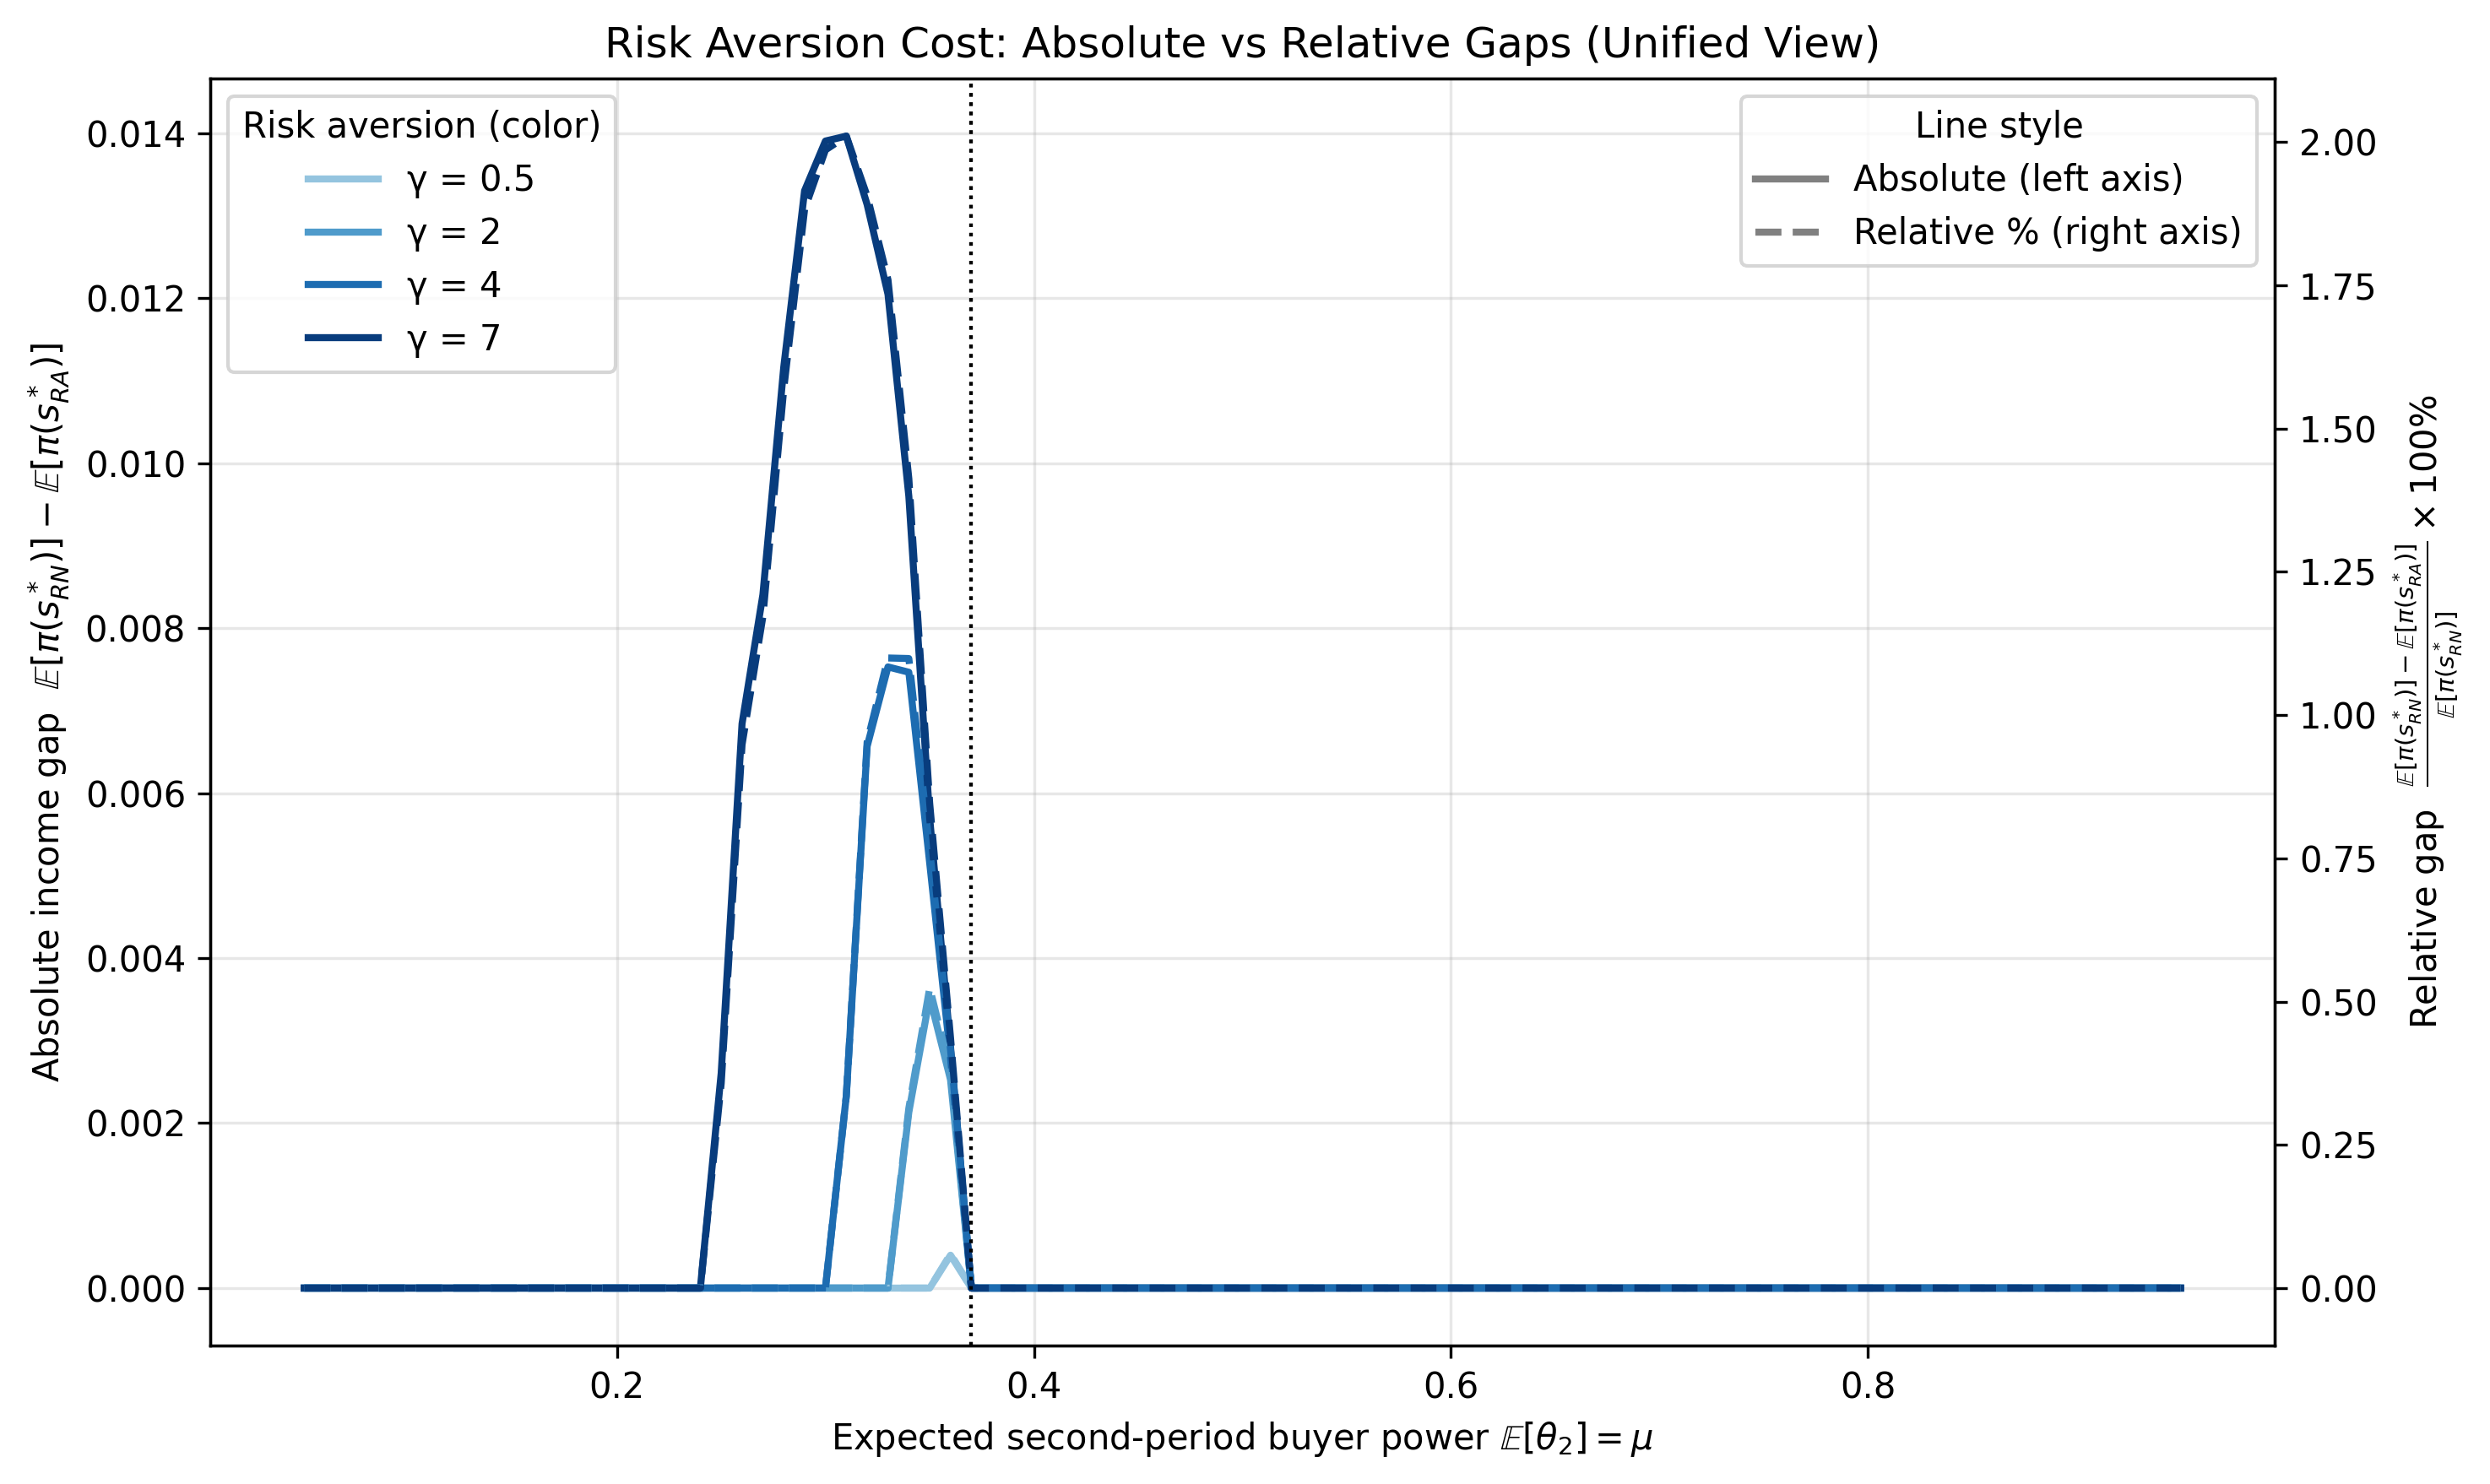
\includegraphics[width=0.85\textwidth]{model_figures/income_gap_vs_mu_(unified).png}
    \caption{Absolute and relative expected income losses from risk aversion. 
    Solid lines show the absolute gap $\mathbb{E}[\pi(s^*_{RN})]-\mathbb{E}[\pi(s^*_{RA})]$ (left axis). 
    Dashed lines show the same gap as a percentage of the risk-neutral benchmark (right axis). 
    Colors indicate the degree of risk aversion ($\gamma$). 
    The vertical dotted line marks the risk-neutral switching threshold $\mu^\star$ where storage ceases to be profitable.}
    \label{fig:unified_gap_plot}
\end{figure}


\textbf{Quantitative illustration.} Simulation results (Figure~\ref{fig:unified_gap_plot}) show that absolute income losses from risk aversion peak at roughly 0.02--0.03 in normalized units, while the relative gap reaches about 2 percent of expected income under strong risk aversion ($\gamma=7$) and falls below 1 percent for moderate values ($\gamma=2$ to $4$). These effects vanish when storage is clearly profitable or clearly unprofitable, underscoring that the ``cost of risk aversion'' is concentrated exactly at the margin where storage incentives are fragile.

\textbf{Interpretation.} The income effect from lowering risk aversion is modest in size but targeted: it recovers the ``money left on the table'' precisely where risk aversion binds most. Instruments that ease liquidity risk (warehouse-receipt finance, seasonal credit lines), transfer income across states (crop insurance), or smooth consumption (safety nets) can move farmers measurably closer to the risk-neutral storage decision. Even modest financial deepening---for example, reducing effective $\gamma$ from 7 to 2---eliminates more than half of the small but systematic income gap in this calibration.





\subsection{Synthesis}

Competition, storage efficiency, and risk-sharing operate through distinct mechanisms but share a common outcome: higher expected incomes without direct price supports. The examples above show that (i) improving competition today or tomorrow, (ii) raising $\kappa$ by 10\%, and (iii) lowering effective $\gamma$ all yield measurable gains---often by triggering discrete shifts in storage. As such, these tools expand the policy frontier, complementing traditional interventions while avoiding many of their well-known downsides.





\section{Conclusion}
\noindent This chapter demonstrates that storage adoption can have a dynamic impact on the welfare of farmers facing oligopsony power, providing inter-temporal arbitrage opportunities and stronger bargaining power over time. Cold storage adoption helps farmers overcome trading-time limitations and benefit even from temporal changes in trader competition alone. Examining storage from a market competition perspective offers a fresh approach to analyzing the influence of inventory on growers' and sellers' marketing strategies and their bargaining power.

My baseline model provides a theoretical basis for small-scale farmers' storage and marketing choices in developing countries. It focuses on farmers' intra-seasonal strategies and the storing-decision process, where farmers observe farm-gate prices and market structure at harvest and decide whether to immediately sell some, all, or none of their crops. When farmers have insufficient bargaining power at a single point in time, the adoption of storage at lower storage costs would give them inter-temporal arbitrage opportunities. 


This chapter's application extends beyond the fresh apple industry to various settings. Cold storage and inventory play a crucial role in agricultural transactions, commonly serving as tools for sellers to take advantage of demand-driven price fluctuations. However, the competitive dynamics among buyers (middlemen) can vary over time, even without changes in demand or supply elsewhere in the industry chain. By examining storage from a market competition perspective, this model offers a fresh approach to analyzing the influence of inventory on growers' and sellers' marketing strategies and their bargaining powers in agricultural commodity industries.

In many developing countries, governments could complement or even substitute for minimum purchase price programs and direct cash transfers by subsidizing farmers' investment in storage infrastructure. Rather than intervening directly in output markets, such policies would expand farmers' access to quality-preserving storage technologies, enabling them to choose when to sell their crops. By shifting sales to more favorable periods, farmers can strengthen their bargaining position against middlemen, while the resulting improvements in market efficiency benefit both producers and consumers along the supply chain.





% %---------------------------%
% \newpage
% \section{Memo: A Difficult Tradeoff between Two Utility Aggregation Approaches}
% \noindent As I finalize revisions on the current model, I identify a major conceptual drawback: the optimal storage share becomes increasing in the farmer's degree of risk aversion when the expected second-period buyer power is higher than the first-period level. In other words, the model implies that farmers who expect a worse market condition in the future would store more if they are more risk-averse. This result is counterintuitive and lacks a clear behavioral or economic justification.

% This inconsistency has prompted me to revisit an alternative formulation we previously considered. Specifically, we face a fundamental modeling choice between:
% \begin{itemize}
%     \item Maximizing the expected sum of discounted utilities of income, versus
%     \item Maximizing the utility of the sum of discounted incomes.
% \end{itemize}
% Both approaches are theoretically sound but carry distinct implications. Below, I outline the tradeoffs between the two so we can more clearly evaluate the direction forward.

% \subsection{Current Setting: Sum of Discounted Utilities of Income}

% \noindent This is the standard formulation in intertemporal utility theory, where utility is evaluated separately in each period and future utility is discounted by a factor $\delta$:
% \begin{equation}
% \max_{s \in [0,1]} ; U\left((1 - s) p_1\right) + \delta \cdot \mathbb{E} \left[ U\left(s \cdot p_{2,\text{net}} \right) \right].
% \end{equation}

% \noindent Key assumptions and implications:
% \begin{itemize}
% \item Utility is additive and separable across time.
% \item The agent is risk-averse within each period, but not across periods.
% \item This structure implies a preference for income smoothing over time.
% \end{itemize}

% The primary advantage of this formulation lies in its analytical tractability. The separability allows us to derive a closed-form solution for the optimal storage share $s^*$, even under nontrivial distributional assumptions about future buyer power. It fits neatly within the expected utility framework and supports comparative statics analysis with intuitive results, except for the key case of higher second-period buyer power involving risk aversion.

% Through simulation and sensitivity checks (see Figure), I observe a troubling result: when expected second-period buyer power is pessimistic ($\theta_2$ is larger), the optimal storage share becomes increasing in risk aversion. This is counterintuitive. Typically, greater risk aversion should lead agents to reduce exposure to future uncertainty—i.e., store less. This expected behavior holds in the left region of the figure (where expectations about the future are optimistic), but breaks down in the right region.

% Upon closer inspection, this anomaly stems from the fact that the model assumes risk aversion only within periods. The framework lacks intertemporal risk aversion—i.e., there is no mechanism to penalize uncertainty in total income across periods. Unless we fundamentally alter the utility function (e.g., by adopting a non-additive or piecewise utility structure), this counterintuitive outcome cannot be avoided within this setting.

% One might ask how prior literature addresses this. The answer is: they often avoid it by making restrictive assumptions or narrowing the scope of analysis. For instance, \citet{ruhinduka2020smallholder} (the work by Travis Lybbert and his co-authors studying the post-harvest storage decisions) assume $\mathbb{E}(p_2) > p_1$, ensuring that $\partial s^* / \partial \gamma < 0$, thus sidestepping the unintuitive regime altogether.


% \subsection{Alternative Setting: Utility of the Sum of Discounted Income}
% \noindent This alternative formulation, similar to the structure used in your work with Saitone and Malan \citep{saitone2018price}, applies the utility function to the entire stream of income, aggregated and discounted to the present:
% \begin{equation}
% \max_{s \in [0,1]} ;\mathbb{E} \left(U\left[ (1 - s) p_1 + \delta \cdot s \cdot p_{2,\text{net}} \right]\right).
% \end{equation}

% \noindent Key assumptions and implications:
% \begin{itemize}
% \item Utility is applied to the total discounted income as a single aggregated payoff.
% \item The agent exhibits intertemporal risk aversion—preferences depend on risk in the total income stream, not just within each period.
% \item This formulation is commonly used in investment and project evaluation models, especially under uncertainty.
% \end{itemize}

% The primary strength of this setting is its consistency with empirical observations. Simulations under a CRRA utility specification (see Figure show that both risk-neutral and most moderately risk-averse farmers tend to make corner solutions—either storing everything or nothing—which aligns well with real-world behavior. Interior solutions exist but are confined to a narrow region of the parameter space, unlike the smoother, wider range of partial storage outcomes generated by the standard model.

% The main limitation, however, is analytical intractability. Closed-form solutions for the optimal storage share $s^*$ are not available under arbitrary distributions of $\theta_2$ in our case. Solving this model typically requires numerical methods, which restrict our ability to conduct formal comparative statics. An exception arises in cases with a finite number of discrete scenarios—e.g., buyer competition modeled as Bertrand duopoly with known probabilities—in which case closed-form solutions may be derived. Otherwise, we must rely on simulation-based approximation.

% \subsection{3D Visualizations of Both Formulations}

% \noindent I conduct simulations for both utility formulations over a grid defined by the coefficient of relative risk aversion ($\gamma$) and the storage efficiency factor ($\kappa$). The first-period buyer power is fixed at $\theta_1 = 0.6$, and the discount factor is set at $\delta = 1.0$ throughout.

% Figure~\ref{fig:3D_formulation} presents a $4 \times 4$ panel summarizing the simulation results. I examine eight distinct Beta distributions for $\theta_2$, varying in both the mean and variance: two levels of variance—low ($\sigma^2 = 0.02$) and high ($\sigma^2 = 0.05$)—and four values of the mean: $\mu \in {0.2,,0.4,,0.6,,0.8}$.

% \begin{itemize}
%     \item \textbf{Top and Bottom Rows}: These panels display the Beta probability density functions used in the simulations. The top row corresponds to low-variance cases ($\sigma^2 = 0.02$); the bottom row to high-variance cases ($\sigma^2 = 0.05$). Each panel is annotated with the corresponding values of $\mu$, $\sigma^2$, $\alpha$, and $\beta$.
%     \item \textbf{Middle Rows (2 and 3)}: These panels depict the optimal storage share $s^*$ as a 3D surface over the $\gamma$–$\kappa$ grid, conditional on the corresponding $\theta_2$ distribution. The second row shows results under low variance; the third row under high variance.
% \end{itemize}

% Across both formulations, the columns from left to right represent increasing expectations of future buyer power relative to the current level ($\theta_1 = 0.6$):
% \textit{much lower}, \textit{moderately lower}, \textit{approximately equal}, and \textit{much higher}.

% In Figure (corresponding to the sum of discounted utilities formulation), the first two columns align with economic intuition: higher risk aversion leads to lower storage under optimistic expectations, consistent with a dislike of uncertainty. However, in the last two columns—where future buyer power is expected to match or exceed $\theta_1$—the model yields counterintuitive results: only risk-neutral or near risk-neutral farmers avoid storage, while higher risk aversion induces greater storage shares, contrary to standard risk-averse behavior.

% By contrast, in Figure (corresponding to the utility of total discounted income formulation), the patterns are more intuitive. In the third and fourth columns—where second-period buyer power is expected to be comparable to or stronger than in the first period—nearly all farmers choose not to store at all ($s^* = 0$), regardless of risk preferences. This outcome reflects a stronger aversion to future uncertainty at the level of total income, and the model's capacity to rationalize boundary decisions aligns more closely with observed behavior.




% \subsection{Decision Point: Selecting the Modeling Framework}

% \noindent In summary, we face a fundamental modeling choice going forward. Each option carries significant tradeoffs in terms of interpretability, tractability, and alignment with empirical behavior:

% \begin{enumerate}
%     \item \textbf{Maintain the current formulation}—maximize the expected sum of discounted utilities of income.
% This approach is analytically tractable and allows for closed-form solutions and comparative statics. However, it yields a counter-intuitive prediction: under pessimistic expectations for future buyer power, more risk-averse farmers are predicted to store more, not less. Proceeding with this model requires us to develop a compelling economic rationale or behavioral interpretation for this result.
%     \item \textbf{Switch to the alternative formulation}—maximize the utility of the sum of expected discounted income.  
% This setting avoids the problematic comparative statics and aligns more closely with observed farmer behavior (e.g., boundary solutions). However, it sacrifices analytical tractability. We would need to rely on simulation-based numerical solutions, or begin with a tractable case (e.g., Bertrand competition with discrete buyer power realizations) and then generalize through approximation.
% \end{enumerate}
